\setchapterpreamble[u]{\margintoc}
\chapter{ViDoRe V3: A Comprehensive Evaluation of Retrieval Augmented Generation in Complex Real-World Scenarios}


\begin{kaobox}[frametitle=Paper Abstract]
Retrieval-Augmented Generation (RAG) pipelines must address challenges beyond simple single-document retrieval, such as interpreting visual elements (tables, charts, images), synthesizing information across documents, and providing accurate source grounding. Existing benchmarks fail to capture this complexity, often focusing on textual data, single-document comprehension, or evaluating retrieval and generation in isolation. We introduce \textbf{\vidorev}, a comprehensive multimodal RAG benchmark featuring multi-type queries over visually rich document corpora. It covers 10 datasets across diverse professional domains, comprising ~26,000 document pages paired with 3,099 human-verified queries, each available in 6 languages. Through 12,000 hours of human annotation effort, we provide high-quality annotations for retrieval relevance, bounding box localization, and verified reference answers. Our evaluation of state-of-the-art RAG pipelines reveals that visual retrievers outperform textual ones, late-interaction models and textual reranking substantially improve performance, and hybrid or purely visual contexts enhance answer generation quality. However, current models still struggle with non-textual elements, open-ended queries, and fine-grained visual grounding. To encourage progress in addressing these challenges, the benchmark is released under a commercially permissive license.

\end{kaobox}

\section{Introduction}

\begin{figure*}[h]
    \centering
    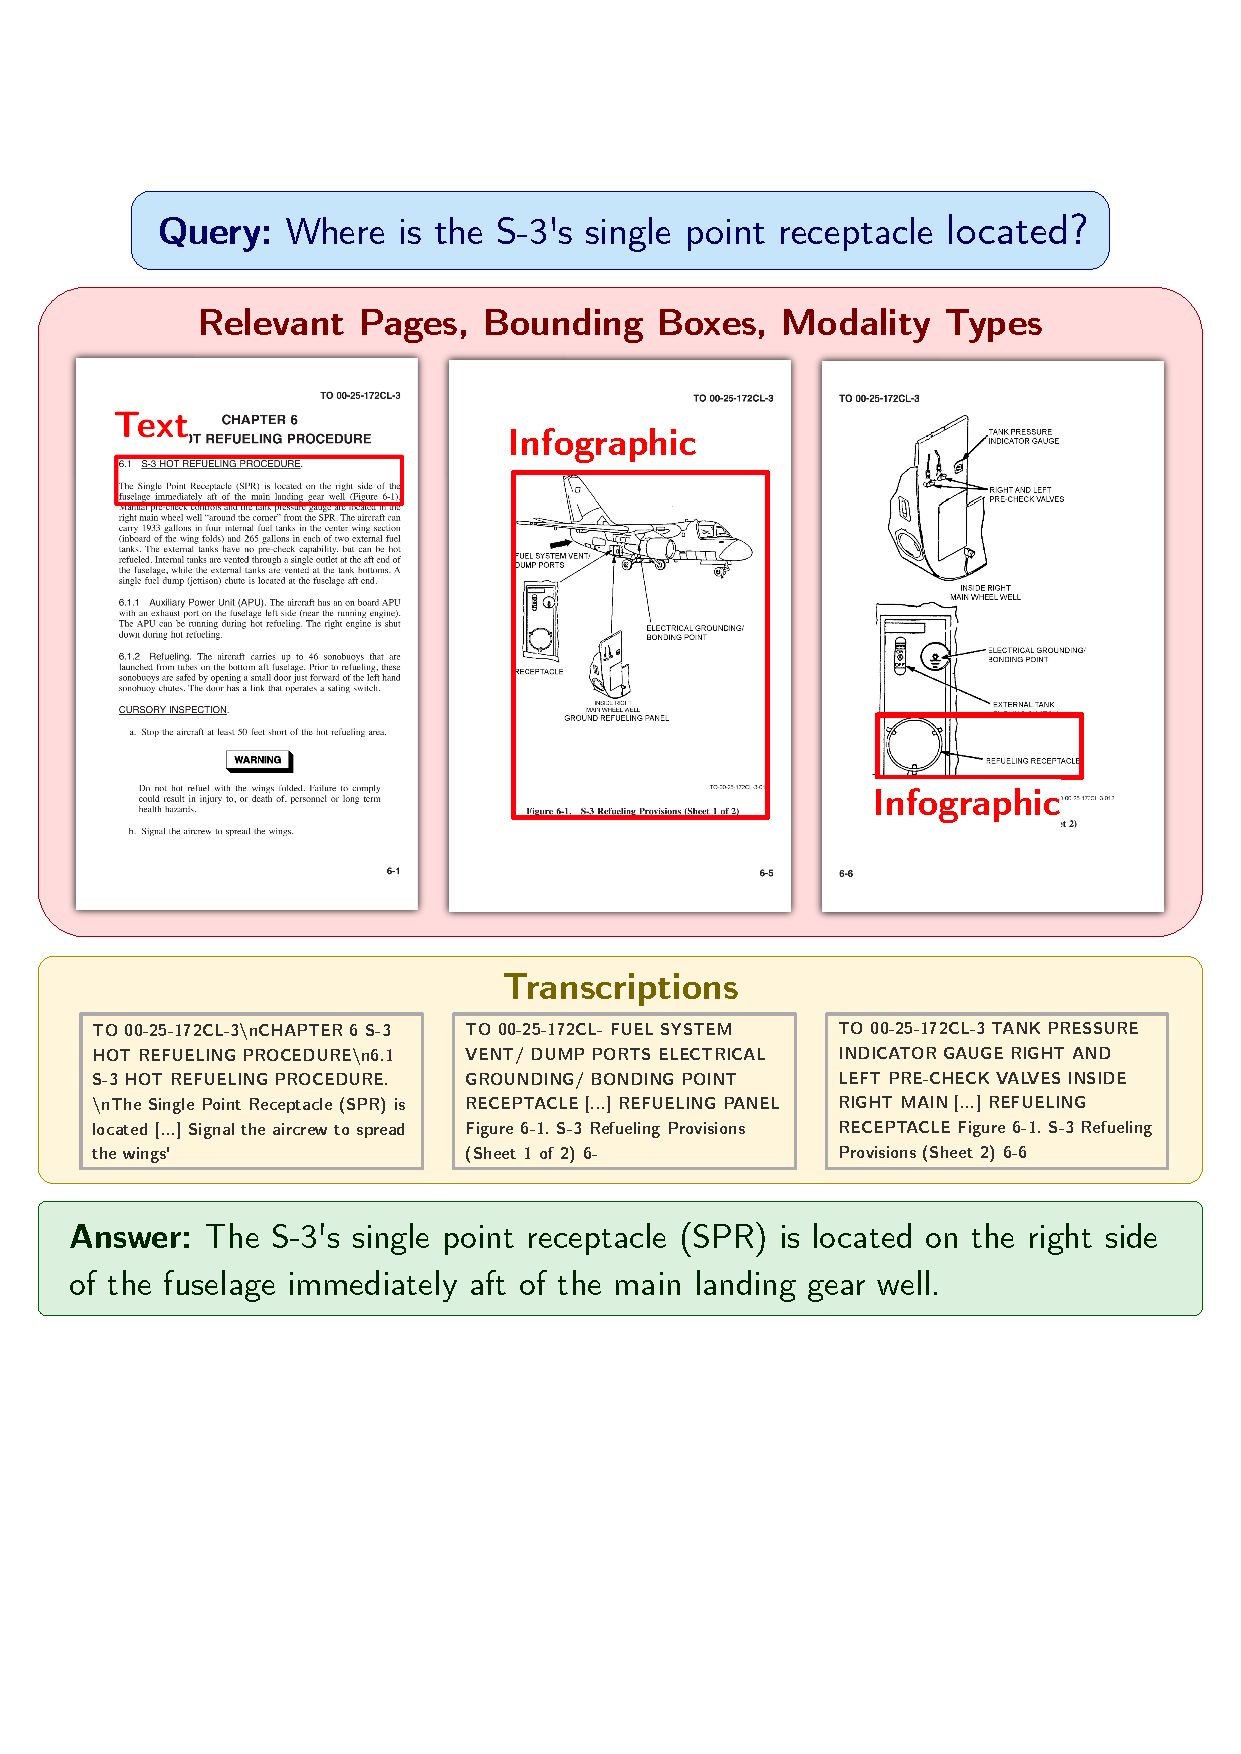
\includegraphics[trim={2cm 6.5cm 2cm 3.5cm}, clip, width=0.9\textwidth]{images/vidorev3_images/vidore_sample.pdf}
    \caption{\textbf{ViDoRe V3 sample.} Each query is annotated with the relevant pages, a document-grounded answer, bounding boxes localizing supporting evidence and modality labels for each bounding box. Documents are provided in image, text and PDF formats.} % TODO: clean this caption
    \label{fig:sample}
\end{figure*}

% In these settings, accurate information retrieval offers the highest operational value yet faces the most unstructured, heterogeneous data. That is why, real-world pipelines must tackle challenges that extend beyond single-document textual retrieval.

Retrieval-Augmented Generation (RAG) \sidecite{lewis2021retrievalaugmentedgenerationknowledgeintensivenlp} has become the dominant paradigm for knowledge-intensive NLP tasks \sidecite{gao2024retrievalaugmentedgenerationlargelanguage, fan2024surveyragmeetingllms}. Yet practical deployments introduce complexities that academic benchmarks often overlook when focusing on single-document textual retrieval. First, documents encode critical information in visual elements such as tables, charts, and images designed for human interpretation, which text-only pipelines often ignore \sidecite{abootorabi2025askmodalitycomprehensivesurvey, cho2024m3docragmultimodalretrievalneed}. Second, user queries often require open-ended synthesis, comparison, and reasoning over scattered information, not simple factoid lookup \sidecite{tang2024multihopragbenchmarkingretrievalaugmentedgeneration, conti2025contextgoldgoldpassage, thakur2025freshstackbuildingrealisticbenchmarks}. Third, trustworthy systems must ground responses to specific source locations (e.g., bounding boxes), to mitigate hallucinations \sidecite{gao2023enablinglargelanguagemodels, ma2024visaretrievalaugmentedgeneration}.

Existing benchmarks leave these requirements only partially addressed. Early Visual Document Understanding (VDU) benchmarks focus on single-page comprehension, ignoring the complexity of large document corpora \sidecite{mathew_docvqa_2020}. Recent retrieval-centric benchmarks do not evaluate generation quality and grounding \sidecite{faysse2025colpaliefficientdocumentretrieval,günther2025jinaembeddingsv4universalembeddingsmultimodal}. Some multimodal datasets attempt to bridge this gap but rely on extractive, short-answer tasks that fail to exercise complex reasoning \sidecite{cho2024m3docrag}, or lack multilingual diversity and fine-grained visual grounding \sidecite{peng2025unidocbenchunifiedbenchmarkdocumentcentric}.

\begin{figure*}[t!]
    \centering
    % \includegraphics[trim={0cm 2cm 0cm 2cm}, clip, width=\textwidth]{images/vidorev3_images/test-vidore-v0.png}
    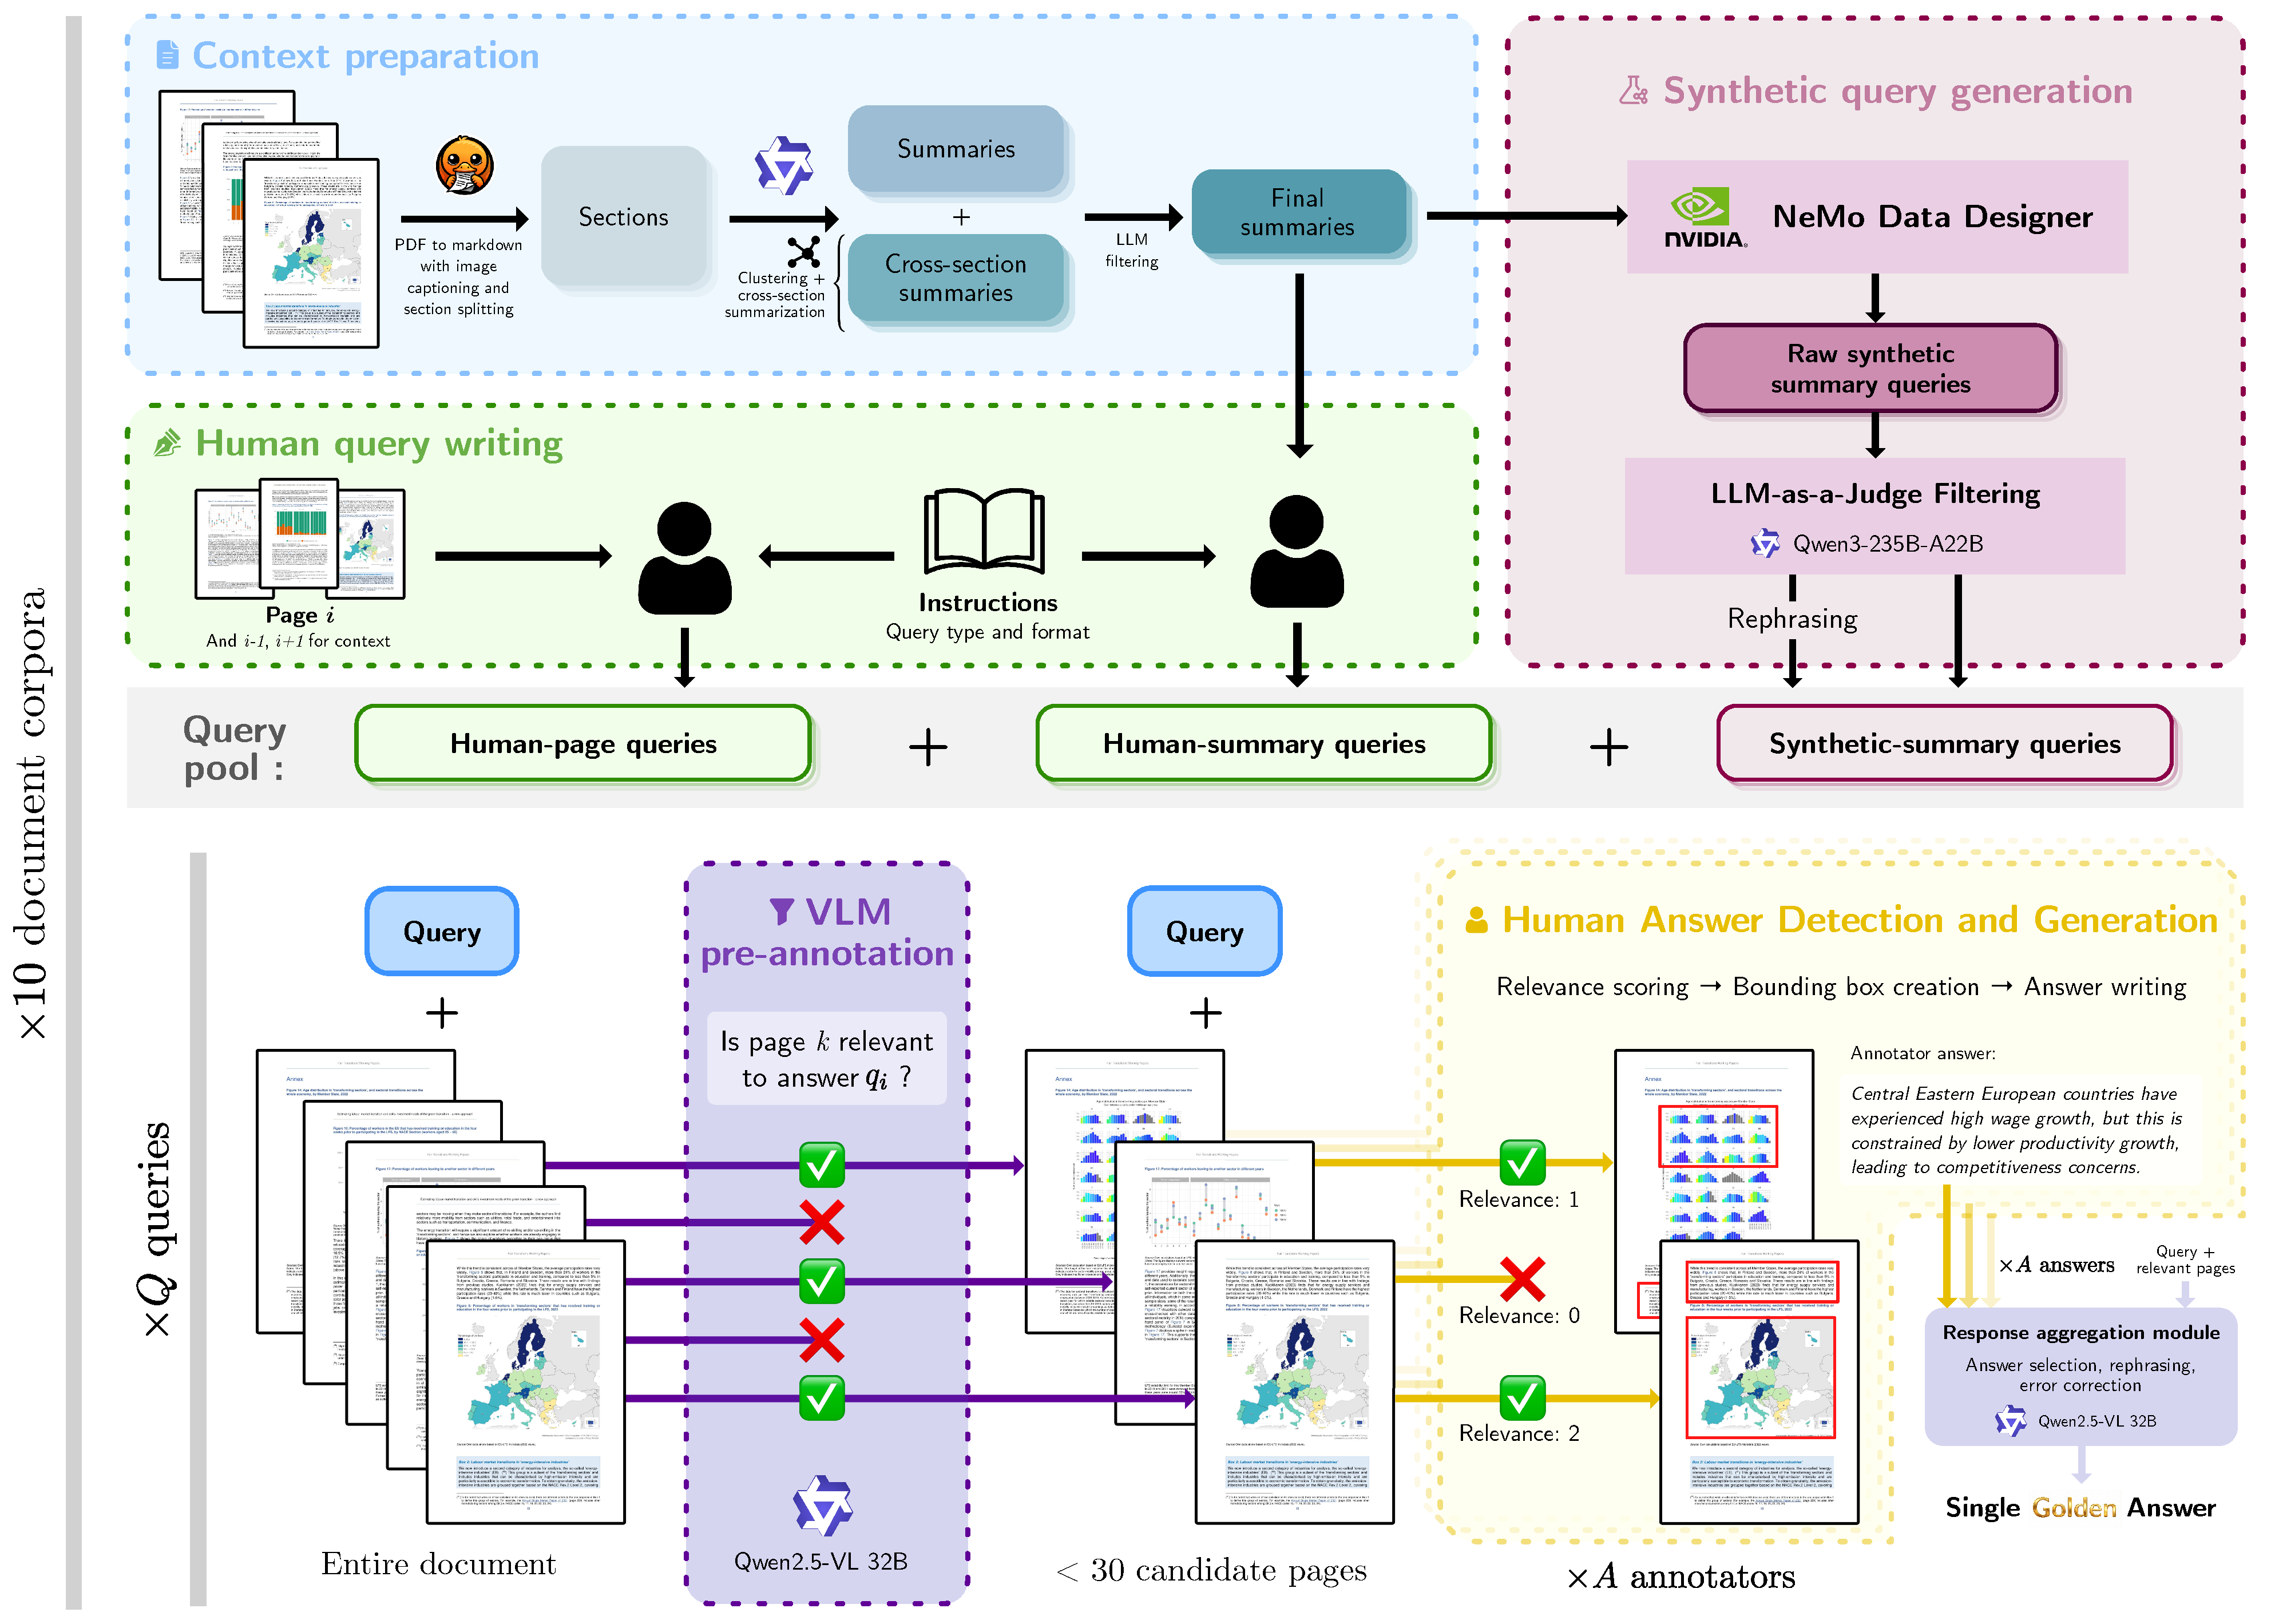
\includegraphics[width=\textwidth]{images/vidorev3_images/dataset-generation-vf.pdf}
    \caption{\textbf{Overview of the benchmark creation process.} Queries are sourced from 3 streams: \textit{human extractive} (using raw pages), \textit{human blind contextual} (using summaries to mitigate extractive bias), and \textit{synthetic blind contextual}. For each query, a VLM pre-filtered subset of candidate pages is labeled by 1--3 human annotators that perform relevance scoring, bounding box localization and answer generation. A final response aggregation combines annotator answers into a single answer.} %\gmor{Could you identify in the main figure what are Tasks 1 and Task 2?}\anto{Yes, it would be great to reuse the terms Query Writing and Query Linking}}
    \label{fig:full process}
\end{figure*}

To address these limitations, we introduce \textbf{\vidorev}, a benchmark designed for complex and realistic end-to-end RAG evaluation on visually rich document corpora. Our contributions are:

% A Scaled Human-in-the-Loop ... (pas ouf, j'aime bien le realistic mais tous les titres deviennent trop longs) on a un peu de place ici
% A Novel Human... methodo for realistic/complex? queries
% From Claude: One small consideration: some reviewers find "novel" unnecessary since contributions are expected to be new. pas faux
\paragraph{1. A Human Annotation Methodology for Realistic Queries} We propose an annotation protocol for generating diverse queries and fine-grained query-page annotations. By restricting annotator access to document content during query formulation, we capture authentic search behaviors and mitigate bias toward simple extractive queries. Vision-Language Model (VLM) filtering combined with human expert verification enables efficient, high-quality annotation at scale.

%\paragraph{1. A Complete Human-in-the-Loop Annotation Methodology.} We introduce a novel human-in-the-loop methodology designed to capture authentic information-seeking behaviors rather than simple fact-verification. By restricting the information available to annotators during query formulation, we mitigate the bias toward trivial, purely extractive questions. This protocol combines Vision-Language Model (VLM) pre-filtering with expert human verification to efficiently produce high-quality retrieval relevance, bounding box grounding, and verified reference answers at a significant scale.
% \paragraph{1. A Complete Human-in-the-Loop Annotation Methodology.} We introduce a novel annotation protocol that combines Vision-Language Model (VLM) pre-filtering with expert human verification. This methodology allows for the creation of high-quality, fine-grained annotations \manu{at large scale? / processing large volumes of data to select from?}. It includes retrieval relevance, bounding box grounding, and verified reference answers at a scale and depth previously unattained for complex document tasks. \anto{maybe a bit too enthusiastic}
\paragraph{2. The ViDoRe V3 Benchmark} Applying this methodology to 10 industry-relevant document corpora, we build ViDoRe V3, a multilingual RAG benchmark comprising ~26,000 pages and 3,099 queries, each available in 6 languages. Two datasets are held out as a private test set to mitigate overfitting. The public datasets are released under a commercially permissive license.  %The benchmark is fully integrated into the MTEB ecosystem and leaderboard \sidecite{muennighoff2023mteb}, and the public datasets are released under a commercially permissive license.
\paragraph{3. Comprehensive Evaluation and Insights} Leveraging our granular annotations, we benchmark state-of-the-art models on \textbf{(i)} retrieval accuracy by modality and language, \textbf{(ii)} answer quality across diverse retrieval pipeline configurations, and \textbf{(iii)} visual grounding fidelity. Our analysis surfaces actionable findings for RAG practitioners.


% \anto{Gautier's comment: Add in intro a sentence / short paragraph of why we focus on "enterprise" (realistic, where IR has the most value, difficult, messy, ...), if this wording is used throughout the text} Retrieval-Augmented Generation (RAG) \sidecite{lewis2021retrievalaugmentedgenerationknowledgeintensivenlp} is now a widely adopted paradigm for knowledge-intensive Natural Language Processing (NLP) tasks  over large document corpora  \sidecite{gao2024retrievalaugmentedgenerationlargelanguage, fan2024surveyragmeetingllms}. However, RAG pipelines deployed in enterprise settings must tackle challenges that extend beyond single document textual retrieval \sidecite{cho2024m3docragmultimodalretrievalneed}. Documents encode critical information in visual elements such as tables, charts, and images designed for human interpretation \sidecite{abootorabi2025askmodalitycomprehensivesurvey}. Additionally, many realistic queries are open-ended, requiring the synthesis, comparison, or explanation of information scattered across multiple documents rather than simple factual answers \sidecite{yang2018hotpotqadatasetdiverseexplainable, wang2023knowledgegraphpromptingmultidocument, tang2024multihopragbenchmarkingretrievalaugmentedgeneration, thakur2025freshstackbuildingrealisticbenchmarks}. \manu{Useful references might include FreshStack (Thakur) that recognize many of the pitfalls in IR benchmarks. The paper might be a nice source of inspiration fot some other refs (and it's quite likely one of the authors is reviewer here).} A further challenge lies in ensuring that generated responses can be reliably traced back to specific source locations within documents, which becomes particularly complex when dealing with visual content rather than plain text \sidecite{gao2023enablinglargelanguagemodels, ma2024visaretrievalaugmentedgeneration}.

% % \begin{figure*}[t!]
% %     \centering
% %     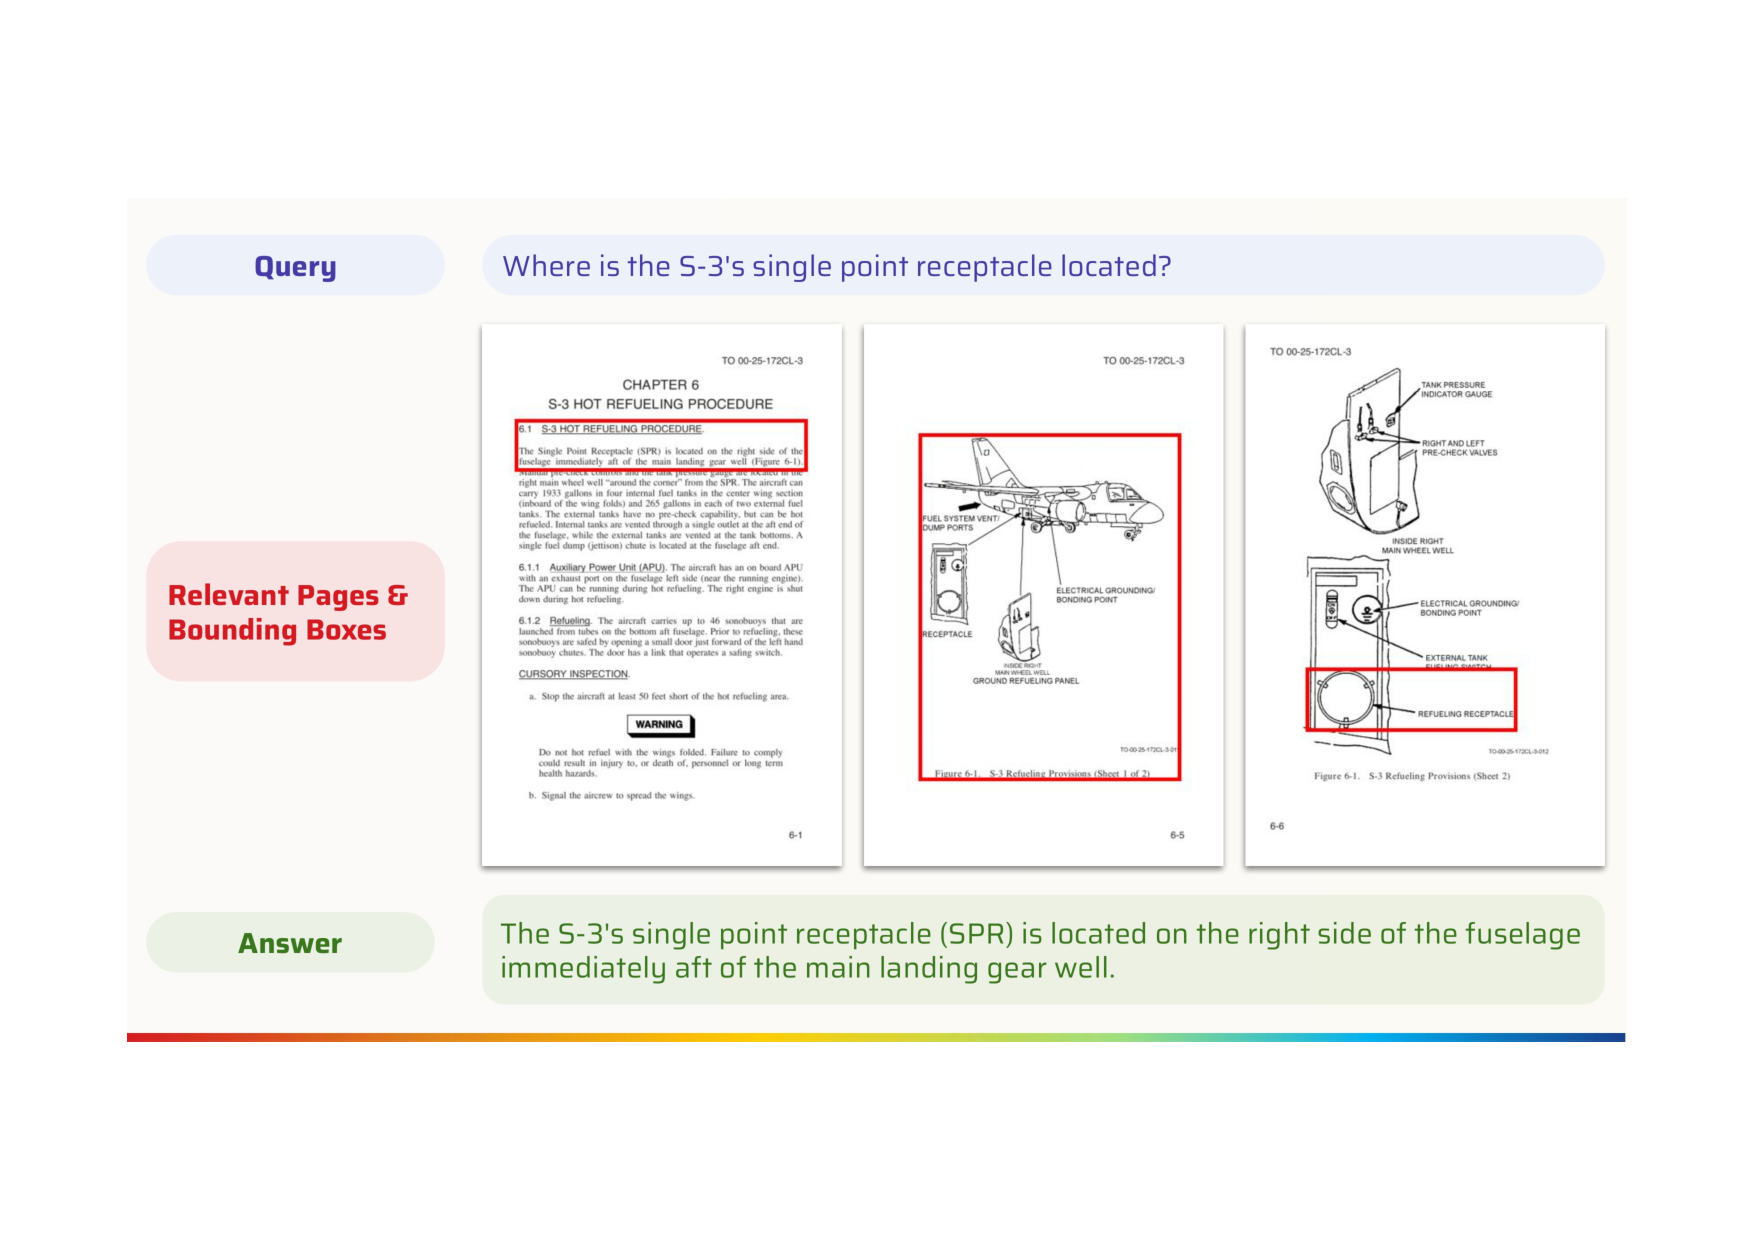
\includegraphics[trim={0cm 2cm 0cm 2cm}, clip, width=\textwidth]{images/vidorev3_images/dataset_overview.pdf}
% %     \caption{\anto{Placeholder for benchmark overview figure, make it single column if possible} \vic{We can use Antoine's figure as the main figure? Just being cautious about the limited space we have}\anto{Examples of samples are mandatory in a benchmark paper like this, I think we can do a single column figure to make it fit cf. \href{here}{https://arxiv.org/pdf/2007.00398}}}
% %     \label{fig:full process}
% % \end{figure*}

% \que{More focus on VISUAL retrieving}\que{need to introduce MM-RAG in the abstract}

% %To address these challenges, we need detailed annotations that cover the 3 main tasks of a MM-RAG pipeline: multimodal retrieval (finding the most relevant contexts for a given query), answer generation (generating an answer to the query based on a set of retrieved contexts) and answer grounding (localizing the parts of the documents that mention the answer to the query). \vic{imo we can remove this paragraph}
% % TODO: rewrite this paragraph well

% However, existing datasets largely fail to capture this end-to-end complexity. Early visual visual document understanding datasets \sidecite{mathew_docvqa_2020, wang2024charxiv} focus primarily on single-page comprehension, ignoring the retrieval challenges of large corpora. Conversely, recent retrieval-centric benchmarks \sidecite{faysse2025colpaliefficientdocumentretrieval, macé2025vidorebenchmarkv2raising, günther2025jinaembeddingsv4universalembeddingsmultimodal} isolate the search component, overlooking the subsequent generation and grounding quality. DUDE \sidecite{van2023document} and M3DocRAG \sidecite{cho2024m3docrag} extend evaluation to multi-page settings but remain largely extractive, emphasizing short factoid answers over the multi-step reasoning and synthesis demanded by open-ended enterprise queries. While contemporary works such as UniDocBench \sidecite{peng2025unidocbenchunifiedbenchmarkdocumentcentric} have made strides toward end-to-end evaluation including summarization tasks, they remain limited to a single language and lack visual grounding annotations necessary to diagnose hallucination in complex layouts. Some benchmarks \sidecite{ma2024visaretrievalaugmentedgeneration, yu2025bboxdocvqalargescale} address the issue of visual grounding but they are far from enterprise domains.
% % While early multimodal benchmarks have attempted to provide ways of evaluating these tasks, they often fail to capture the full complexity of enterprise-level RAG. Document-based question answering benchmarks such as DocVQA \sidecite{mathew_docvqa_2020} and CharXiv \sidecite{wang2024charxiv} focus primarily on single-image understanding. More recent datasets, including M3DocVQA \sidecite{cho2024m3docrag} and DUDE \sidecite{van2023document}, extend to multi-page documents but remain largely extractive, emphasizing short answers that do not stress multi-step reasoning or synthesis. Recent document retrieval benchmarks \sidecite{faysse2025colpaliefficientdocumentretrieval, macé2025vidorebenchmarkv2raising} isolate retrieval performance, largely overlooking answer generation quality, grounding fidelity, and query diversity. Among contemporary works, UniDocBench \sidecite{peng2025unidocbenchunifiedbenchmarkdocumentcentric} offers the most significant end-to-end evaluation across industry domains; however, it remains constrained by a focus on extractive questions and a single language. \anto{Not really just extractive, they also have summarization and comparison}

% To address this gap, we introduce the following contributions:
% % \manu{Bullet points are a waste of paper space, you won't find them a lot in most papers cause it means you had space to spare}
% \paragraph{Contribution 1} We release \textbf{ViDoRe V3}, a comprehensive RAG benchmark emphasizing open-ended queries on long-form, visually rich document corpora. It is composed of 10 datasets from diverse industry domains, totaling about 26,000 document pages paired with 3,099 unique queries available in 6 languages. \manu{do we want to include something about the fact is representative of existing RAG use cases ? ie. domains are diverse but also carefully chosen} It contains fine-grained expert \que{is the expert ok here?} human annotations developed through a 12,000-hour annotation process, including relevant page annotations for retrieval, bounding boxes for visual grounding, and verified reference answers (Section~\ref{sec:benchmark creation}).
% \paragraph{Contribution 2} Using benchmark annotations, we evaluate \textbf{(i)} retrieval accuracy, providing insights into the effects of pipeline modality, query language and type, and context modality and length (Section~\ref{sec:retrieval results}), \textbf{(ii)} final answer generation and how it varies with retrieval pipeline design choices (Section~\ref{sec:visual grounding results}), \textbf{(iii)} visual grounding based on bounding box localization accuracy (Section~\ref{sec:visual grounding results}). \manu{Contrib 1 is meant to enable this so this is not a contribution on its own. what is a contribution is to evaluate "current models / current pipelines to gather actionnable practicle insights". }

% \manu{I believe one of the selling points and the novelty of this paper lies in the "method" behind the annotation and this is what we can insist in as a contribution. Figure 2 perfectly goes with my point here."Novel methodology to produce high quality RAG annotations at scale using human in the loop and AI agents etc etc. Remember that Vidore v2 was never published so all contribs of v2 can be used in this paper directly I believe this "methodology as a novelty" angle is the one that will be of interest to the ACL reviewers. Personnaly, this would be contrib 1 to me, then the benchm,ark as 2, then the insights as 3 --> clear storyline.}

% \anto{Gautier's comment: Vidore V2 is on arxiv so not sure we can reuse them as contributions of this paper}
% \que{Don't think VidoreV2 being on arxiv prevents us from describing this as a contribution, the approach is much more fine grained and tuned than for v2 (with actual human in the loop, and not just an António in the loop)}

% \paragraph{Contribution XXX} \que{Construction work :} We describe a new human-in-the-loop annotation process for realistic end-to-end RAG benchmark combining pre-filtering via VLM into fine grained human annotations. We purposedly limit information available at query generation time to prevent query being really specific or plainly extractive. 


% To foster community adoption, ViDoRe V3 is fully integrated in the MTEB \sidecite{muennighoff2023mteb} ecosystem. Retrieval results are publicly available on a dedicated MTEB leaderboard\footnote{\href{https://mteb-leaderboard.hf.space/?benchmark_name=ViDoRe(V3)}{Leaderboard link} \gmor{I think we should make the URL explicit here, as the paper might be printed}\que{I think the link should be anonymous for submission} \anto{YES}}. 


% \begin{table*}[t]
% \small
% \centering
% \renewcommand{\arraystretch}{0.9}
% \begin{tabular}{p{2cm}cccccc}
% \toprule
% & \makecell{\textbf{MMLongBench} \\ \scriptsize\sidecite{ma2024mmlongbenchdocbenchmarkinglongcontextdocument}}
% & \makecell{\textbf{MIRACL-VISION} \\ \scriptsize\sidecite{osmulski2025miraclvisionlargemultilingualvisual}} & \makecell{\textbf{JinaVDR} \\ \scriptsize\sidecite{günther2025jinaembeddingsv4universalembeddingsmultimodal}} & \makecell{\textbf{Vidore V1} \\ \scriptsize\sidecite{faysse2025colpaliefficientdocumentretrieval}} & \makecell{\textbf{Vidore V2} \\ \scriptsize\sidecite{macé2025vidorebenchmarkv2raising}} & \makecell{\textbf{ViDoRe V3} \\ \scriptsize(this work)} \\
% \midrule
% PDF Documents & \Checkmark &  & \partially & \partially & \Checkmark & \Checkmark \\ \midrule
% % Different Query Types & \questionmark & \questionmark & \questionmark & \questionmark & \questionmark & \questionmark & \Checkmark \\ \midrule
% % Different Query Formats & \questionmark & \questionmark & \questionmark & \questionmark & \questionmark & \questionmark & \Checkmark \\ \midrule
% Multi page Queries & \Checkmark & Sometimes & Sometimes & & \Checkmark & \Checkmark \\ \midrule
% Multi document Queries & & & & & & \Checkmark \\ \midrule
% Answers & \Checkmark & & & & & \Checkmark \\ \midrule
% Grounding Bounding Boxes &  & & & & & \Checkmark \\ \midrule
% Human Verification & \Checkmark & & \partially & & \Checkmark & \Checkmark \\ \midrule
% Commercially Open License & & \Checkmark & & \partially & & \Checkmark \\ \midrule
% Average retrieval space & \questionmark & \questionmark & \questionmark & \questionmark & \questionmark & \questionmark \\ \midrule
% Number of pages per query & \questionmark & \questionmark & \questionmark & \questionmark & \questionmark & \questionmark \\
% \bottomrule
% \end{tabular}
% \caption{Comparison of Visual Retrieval Benchmarks. \anto{Should I add this benchmark \href{https://huggingface.co/datasets/llamaindex/vdr-multilingual-test}{llamaindex benchmark} ?}\anto{How would we add a row for query diversity}\anto{The first row means checks if the corpus is based on real world pdfs}\anto{Maybe we can find a way of presenting }\anto{Improve presentation of criteria column}} % Existing benchmarks don't cover all the criteria for enterprise evaluation
% \label{table:benchmark_comparison}
% \end{table*}

\section{Related Work}

\paragraph{Component-Level Benchmarks (VDU and Retrieval)} VDU has traditionally relied on single-page datasets like DocVQA \sidecite{mathew_docvqa_2020}, alongside domain-specialized variants \sidecite{mathew2021infographicvqa, zhu_towards_2022, wang2024charxiv}. These ignore the multi-page context inherent to RAG. Recent work evaluating bounding-box source grounding \sidecite{yu2025bboxdocvqalargescale} proposes single-page and multi-page tasks but does not address the retrieval component. Conversely, the emergence of late-interaction visual retrievers \sidecite{ma2024unifyingmultimodalretrievaldocument, faysse2025colpaliefficientdocumentretrieval, yu2024visragvisionbasedretrievalaugmentedgeneration, xu2025llamanemoretrievercolembedtopperforming} spurred the creation of retrieval-centric visual benchmarks like Jina-VDR  \sidecite{günther2025jinaembeddingsv4universalembeddingsmultimodal} and \vidore \space V1\&V2  \sidecite{ faysse2025colpaliefficientdocumentretrieval, macé2025vidorebenchmarkv2raising}, but none of these benchmarks jointly evaluate retrieval and answer generation.
% yet no existing visual RAG benchmark jointly evaluates retrieval and answer generation. % faux cf. unidoc bench
%failing to evaluate the downstream generation quality required to synthesize grounded answers.
%While valuable, these ignore the corpus-scale retrieval inherent to RAG; even recent work evaluating bounding-box source grounding \sidecite{yu2025bboxdocvqalargescale} remains confined to single-page contexts.

\paragraph{End-to-End Multimodal RAG} While recent textual RAG benchmarks now capture complex user needs like reasoning or summarizing \sidecite{thakur2025freshstackbuildingrealisticbenchmarks, tang2024multihopragbenchmarkingretrievalaugmentedgeneration, su2024bright}, multimodal evaluation often remains limited to single page queries \sidecite{faysse2025colpaliefficientdocumentretrieval}. Multi-page datasets like DUDE \sidecite{van2023document}, M3DocRAG \sidecite{cho2024m3docragmultimodalretrievalneed}, ViDoSeek \sidecite{wang2025vidorag} or Real-MM-RAG \sidecite{wasserman2025real} prioritize extractive retrieval, lacking the diversity of queries encountered in realistic settings. 
UniDocBench \sidecite{peng2025unidocbenchunifiedbenchmarkdocumentcentric} represents a concurrent effort that similarly addresses diverse query types and provides comparative evaluation across multiple RAG paradigms. While this benchmark offers valuable contributions, it relies on synthetically generated queries via knowledge-graph traversal, is restricted to English documents, and constrains grounding annotations to parsed document elements. In contrast, our benchmark offers several complementary strengths: fully human-verified annotations, multilingual coverage, free-form bounding box annotations, and a more systematic evaluation of individual visual RAG pipeline components.

%UniDocBench \sidecite{peng2025unidocbenchunifiedbenchmarkdocumentcentric} is a concurrent benchmark featuring diverse query types and a comparative evaluation of multiple RAG paradigms. However, the queries are synthetically generated via knowledge-graph traversal, the benchmark is English-only, and grounding is limited to parsed document elements. Our benchmark provides fully human-verified annotations, multilingual coverage, free-form bounding boxes, and we conduct more systematic evaluations of visual RAG pipeline components.


\section{Benchmark Creation} \label{sec:benchmark creation}

We design the benchmark to mirror the diversity of information retrieval situations in large-scale realistic environments. To enable pipeline-agnostic evaluation of the 3 core RAG components (retrieval, generation and grounding), while avoiding limitations of synthetic benchmarks, we employ a rigorous three-stage human-in-the-loop annotation process involving document collection, query generation and grounded query answering (\Cref{fig:full process}).

%The goal is to obtain annotations that can help assess the 3 main components of RAG pipelines: information retrieval, answer generation and answer grounding while being agnostic to the type of pipeline used. To avoid problems of preceding synthetic benchmarks and produce high-quality queries, we design a meticulous human annotation involving 3 steps: document collection, query generation and grounded question answering as described by \Cref{fig:full process}.

% TODO: rewrite this paragraph well

\subsection{Document Collection}

We curate 10 diverse corpora by manually selecting openly-licensed documents from governmental, educational, and industry sources, focusing on English and French documents (7 and 3 corpora respectively). The corpora span Finance, Computer Science, Energy, Pharmaceuticals, Human Resources, Industrial Maintenance, Telecom, and Physics. Each features domain-specific terminology and document structures representative of realistic retrieval tasks (details in \Cref{tab:datasets}).
%\footnote{See Appendix \ref{tab:datasets} for corpus details}.

%To reproduce enterprise scenarios and facilitate enterprise adoption, we created the 10 domain corpora by manually selecting documents from governmental, educational and enterprise websites that met our open license criteria. Each corpus focuses on a well-defined domain with specialized terminology and document structures that are representative of real-world industrial document retrieval tasks\footnote{A detailed breakdown of each corpus is provided in Appendix \ref{tab:datasets}.}. Our focus was on a English-French collection, so 7 corpora were selected in English and 3 in French. Domains cover a wide range of enterprise sectors including Finance, Computer Science, Education, Nuclear Energy, Pharmaceuticals, Human Resources, Industrial Maintenance, Telecom and Physics.
% TODO: rewrite this paragraph well

\subsection{Query Generation}

% \paragraph{Query and Task Diversity}
% \que{TODO : merge with 2.3}
% Unlike traditional retrieval benchmarks that treat user intent as monolithic, the benchmark recognizes that complex enterprise queries often layer multiple formats and types. As detailed in Section \ref{sec:query_generation}, we classified queries using a multi-label taxonomy of 7 distinct types across 3 formats.

\paragraph{Query Taxonomy} To evaluate document visual retrieval systems across diverse realistic scenarios, we develop a query taxonomy with two orthogonal dimensions: \textit{Query Type}, defining the user's information need, and \textit{Query Format}, describing the query's syntactic structure. This dual-axis classification enables more nuanced performance analysis than benchmarks focusing solely on interrogative extractive queries. We define 7 Query Types: \textit{open-ended}, \textit{extractive}, \textit{numerical}, \textit{multi-hop}, \textit{compare-contrast}, \textit{boolean}, and \textit{enumerative}, and 3 Query Formats: \textit{question}, \textit{keyword}, and \textit{instruction}. % that reflect modern search engine usage \vic{last part to justify or remove}\footnote{Taxonomy details are described in \Cref{tab:query_taxonomy}}. % To generate even more diverse queries, a synthetic and human query generation processes were followed.

%\paragraph{Query Taxonomy} A primary objective of our benchmark is to evaluate document visual retrieval systems across a comprehensive spectrum of real-world search scenarios. To achieve this, we first develop a detailed query taxonomy that classifies queries along two orthogonal dimensions: \textit{Query Type}, which defines the user's underlying information need, and \textit{Query Format}, which describes the syntactic structure of the query itself. This dual-axis classification allows for a more nuanced analysis of model performance than benchmarks that focus solely on interrogative extractive queries.



% The objective of this benchmark is to get several types of queries that cover different several search engine usages. We listed 7 query categories : 

% \begin{itemize}
%     \item \textbf{open-ended}: an explanatory or descriptive query that synthesizes  information; may be broad in scope and focused on qualitative aspects of the summary,
%     \item \textbf{extractive}: a clear and specific query that can be answered using only a specific piece of information.
%     \item \textbf{compare-contrast}: a query that requires comparing and/or contrasting multiple entities or topics that are closely related to each other
%     \item \textbf{boolean}: a yes/no query that may involve multiple steps of reasoning.
%     \item \textbf{numerical}: a query that asks for a specific number or calculated number given a summary. The query should require more than simply reading numbers directly from the page.
%     \item \textbf{multi-hop}: a complex query that requires retrieving and integrating information from multiple sources or steps to produce a complete answer.
%     \item \textbf{enumerative}: a query that asks to list all examples that possess a common property, optionally requesting details about the specifics of each example.
% \end{itemize}

% Most of the benchmarks focus on interrogative queries. However, modern serach engine users use different query formats. We listed the following:

% \begin{itemize}
%     \item \textbf{question}: a complete sentence that ends with a question mark, typically used to seek specific information or clarification,
%     \item \textbf{keyword}: a brief, often fragmented phrase or set of terms used to search or filter information, without forming a full grammatical sentence.
%     \item \textbf{instruction}: a directive that describes a task to be performed on the documents, often in the form of a command or request.
% \end{itemize}

\paragraph{Context Preparation} We further ensure query diversity by pulling summaries from a heterogeneous set of contexts during the generation process.
%Another way of ensuring query diversity is to pull from a heterogeneous set of contexts during the generation process.
Two types of input contexts are used: specific document sections that target local information retrieval and cross-section summaries that target multi-document context retrieval. These summaries are produced through a refined process inspired by ViDoRe V2 \sidecite{macé2025vidorebenchmarkv2raising}. First, the text is extracted from PDFs using Docling \sidecite{auer2024docling} along with image descriptions. Then, summaries are generated with Qwen3-235B-Instruct \sidecite{qwen3technicalreport} from each document section. They are clustered to group similar summaries together using Qwen3-Embedding-0.6B \sidecite{qwen3embedding} as embedder, UMAP \sidecite{mcinnes2020umapuniformmanifoldapproximation} for dimension reduction and HDBSCAN \sidecite{campello2013density} for clustering. Additionally, cross-section summaries are produced by synthesizing the summaries of 2 to 3 randomly selected sections per cluster. From this pool of summaries, a final subset is curated to maintain a strict balance between single-section and cross-section summaries. The selection also ensures an even distribution across section modalities (text, images, and tables) as defined by the Docling element classification.

\paragraph{Synthetic Query Generation} Queries are generated from the summaries using a first synthetic generation pipeline based on Qwen3-235B. For each summary, a prompt is constructed by sampling a query type and format at random, together with variable attributes such as length and difficulty, in order to promote diversity. The generated queries are subsequently evaluated by the same LLM acting as an automatic judge, which filters outputs according to 4 criteria: information richness, domain relevance, clarity and adherence to query type/format. Finally, 50\% of the retained queries are rephrased to further enhance linguistic variance. This pipeline is implemented using NeMo Data Designer \sidecite{nemo-data-designer} to facilitate generation scaling.

\paragraph{Human Query Writing} Human annotators are provided 2 kinds of contexts: synthetic summaries or specific PDF pages. They are tasked with generating one query following a specific query type and format and one query of their choice that is most adapted to the context provided.

% To generate these diverse query types, several specialized data generation pipelines are developed. For extractive queries, human annotators are provided with specific PDF pages, alongside the preceding and succeeding pages for context, and tasked with generating queries in a predefined format and type. For open-ended queries, we follow a refined process introduced in \sidecite{macé2025vidorebenchmarkv2raising}. 

%2 or 3 sections per cluster are randomly selected and the corresponding summaries are summarized to get cross section summaries. From this pool of summaries, a subset of summaries is selected ensuring that single section and cross section summaries are balanced as well as summaries based on a balanced set of modalities: text, images and tables given by the element classification of Docling. For each summary, we prompt Qwen3-235B-A22B-Instruct-2507 \sidecite{qwen3technicalreport} to generate a query given a predefined type and format. We use an LLM-as-a-Judge to filter the synthetic queries and make sure the distribution follows our needs. We also ask humans to generate queries on  these summaries to get diverse queries from different generation processes. \manu{do humans ever verify the query types and format ? could be nice to mention}

%\manu{This is a big blob of text, maybe simolifying a tad and adding details in the appendix, or structruring this a bit more if ytou decide to make this process as a contribiution (human in the loop blablabla)}

\subsection{Answer Detection and Generation} \label{sec: grounded qa}

Queries are filtered and linked to relevant pages using a hybrid pipeline of VLM pre-filtering and human annotation. It is followed by human answer annotation and visual grounding.

% Once queries are generated, they are meticulously linked to relevant pages and bad quality queries are filtered out. The answer to selected queries is also written by human annotators and bounding boxes are drawn around supporting elements in the documents.

% The objective of this annotation phase is to get the relevant pages containing the answer to the query, the bounding boxes that locate the answer in the pages and the answer to the query. \manu{Link this sentence better with the rest of the process. "Once queries are fenerated, we annotate relecant pages as well as the precise bbox and anszwer that are relevant." I would reference figure 2 a bit more throughout and maybe piggyback on it a bit to simplify exolanations.}


%\manu{simolify pgrhasing: human annotation is intractable. We run a first phase of model-assisted and heuristic filters, relying on qwen XXX to remove pages the model deemed irrelevant given a query, and queries that are too broad. We then transmit the remaining queries and associated pages to expert human annotators to obtain a final XXX}.

\paragraph{Query-Page Linking} Given the scale of our corpora, manual verification of each page relevance for each query is intractable. We therefore adopt a two-stage annotation pipeline. First, Qwen2.5-VL-32B-Instruct \sidecite{qwen25vl} pre-filters candidate pages by assessing whether each page image is relevant to the query. Queries whose answers span more than 30 flagged pages are discarded. Human annotators then review the remaining query-page pairs, evaluating query quality and rating page relevance on a three-point scale (Not Relevant, Critically Relevant, Fully Relevant).

%To facilitate human annotation, we first use the Qwen2.5-VL-32B-Instruct VLM \sidecite{qwen25vl}, which is provided with the query and each page image and tasked with determining whether the page is relevant for answering the query. We then discard queries whose answers are spread across more than 30 pages flagged as relevant. The remaining queries and their candidate pages are reviewed by human annotators to produce the final set of relevant pages. Annotators assess query quality and rate page relevance on a three-point scale (Not Relevant, Critically Relevant, Fully Relevant).

%Extractive queries are annotated by at least one annotator and one reviewer, while more complex non-extractive queries are annotated by at least two annotators and one reviewer. A page is retained as relevant if it is marked as such by either (i) one annotator and one reviewer or (ii) at least two annotators.
% simplifying formulation: we run a first phase of model-assisted and heuristic filters, relying on Qwen2.5-VL-32B-Instruct \sidecite{qwen25vl}.

\paragraph{Relevant Page Selection} To ensure annotation quality, each task is completed by multiple annotators and reviewed by annotation supervisors. Since VLM pre-filtering biases the distribution toward relevant pages, we report Gwet's AC2, as it remains stable under prevalence skew, at 0.760 (see \Cref{appendix: relevance agreement} for dataset-level breakdowns). Given this strong but imperfect agreement, we implement a tiered review process: extractive queries require at least one annotator and one reviewer, while more complex non-extractive queries require at least two annotators and one reviewer. A page is retained as relevant if marked by either (i) one annotator and one reviewer, or (ii) at least two annotators.  %\manu{to me this is a detail that should go in app. here we can say double annotation is used to guarantee quality.}\anto{probably to remove}

%Because pages were pre-filtered by a VLM before human annotation, most pages shown to annotators were likely relevant, creating a skewed class distribution. To address this, we report Gwet's AC2 which remains stable under prevalence skew at $0.760$, on average. Details of agreement metrics by domain are given in appendix \ref{appendix: relevance agreement} Given this score, we ensure a safe relevancy annotation by annotating extractive queries by at least one annotator and one reviewer, while more complex non-extractive queries are annotated by at least two annotators and one reviewer. A page is retained as relevant if it is marked as such by either (i) one annotator and one reviewer or (ii) at least two annotators. \manu{to me this is a detail that should go in app. here we can say double annotation is used to guarantee quality.}\anto{probably to remove}



\paragraph{Answer Generation} For each selected query, annotators were tasked with writing an answer based on the pages they marked as relevant. Given that different annotators might have different answer interpretations and tend not to be exhaustive in their answers, we use Qwen2.5-VL-32B-Instruct to generate a final answer based on the relevant page images marked by the annotators and their answers.

%\paragraph{Inter-Annotator Agreement.} Because pages were pre-filtered by a VLM before human annotation, most pages shown to annotators were likely relevant, creating a skewed class distribution. To address this, we report Gwet's AC2 which remains stable under prevalence skew. On average over all domains, annotators achieved an AC2 of $0.760$. \que{Do we still give the other numbers?}\vic{No but need to add a comment interpreting this metric value}Details of agreement metrics by domain are given in appendix \ref{appendix: relevance agreement}

% To filter most of the irrelevant pages, we use a VLM Qwen2.5-VL-32B-Instruct \sidecite{qwen25vl} that is given the query and each page image in the corpus and asked if the page is relevant to answer the query. After this step, we filter out queries whose answers are dispersed on too many pages, more than 30 flagged pages.
% The remaining queries and the corresponding pages are given to a human annotator that filters the final relevant pages. Queries that are tagged as extractive have at least one annotator and one reviewer and others have at least two annotators and one reviewer, as some annotators might miss relevant pages. Only pages that are tagged as relevant by one annotator and one verifier or at least two annotators are kept as relevant. 

\paragraph{Bounding Boxes and Modality Types}
For each relevant page, annotators delineate bounding boxes around content supporting the query and attribute a modality type to each bounding box: Text, Table, Chart, Infographic, Image, Mixed or Other. 
%This process involves a subjective interpretation of which surrounding context should be included.
Because multiple valid interpretations of bounding boxes can exist, we perform a consistency study to evaluate inter-annotator agreement and establish a human performance upper bound for the task.

We compute inter-annotator agreement on the subset of query-page pairs labeled by two or three annotators. For each annotator, we merge all their bounding boxes into a single zone. We then compare zones across annotators by measuring pixel-level overlap, reporting Intersection over Union (IoU) and F1 score (Dice coefficient). When three annotators label the same sample, we average over all pairwise comparisons.

%\anto{precision, recall, F1 are not the right terminology here. According to Gemini, prefer Inclusion Ratio (A in B), Inclusion Ratio (B in A) and Symmetric Agreement Score or Dice Coefficient} \vic{Gemini tells me it's fine with the changes I made. It's more convenient to have an asymmetric metric for the VLM bounding box evaluation.}

%Across all 10 datasets, we observe a mean IoU of 0.50 and F1 of 0.60, with per-dataset IoU (Table~\ref{tab:inter-annotator bbox agreement}) ranging from 0.44 (Physics) to 0.62 (Pharma) \manu{per dateset stats aere details that could be removed if need be}.

Across all 10 datasets, we observe an average IoU of 0.50 and F1 of 0.60. These moderate agreement scores reflect the inherent subjectivity of the task: annotators typically agreed on the relevant content but differed in granularity (Appendix \ref{appendix: bbox examples}), with some marking tight bounds around specific content while others included surrounding context.

\paragraph{Quality Control} The annotation was conducted by a curated pool of 76 domain-qualified experts with native-level language proficiency. Quality control was performed by 13 senior annotators with enhanced domain knowledge and extensive annotation experience. Detailed protocols regarding the annotator pool and training are provided in Appendix \ref{appendix: annotator pool}.

\subsection{Final Query Distribution} 
% \anto{Move some part to the appendix if not enough space}

We conducted a final human review to remove low-quality queries and resolve labeling ambiguities. \Cref{fig:query_type_distribution} shows the resulting distribution. Extractive queries predominate due to human annotator preference, followed by open-ended queries from targeted sampling. Multi-hop queries were the hardest to scale, suggesting a need for dedicated pipelines. \Cref{fig:content_type_distribution} details page modalities; while text is most prevalent, visual elements like tables, charts, and infographics are well-represented.

% A final review stage was conducted to remove remaining low-quality queries and resolve labeling ambiguities, as some queries could belong to multiple types. The final query type distribution is shown in \Cref{fig:query_type_distribution}. Extractive queries are the most represented, as annotators generally preferred this type. Open-ended queries also appear frequently due to targeted sampling to ensure adequate coverage. Multi-hop queries proved most difficult to generate at scale; producing more high-quality examples of this type would require a dedicated pipeline. \Cref{fig:content_type_distribution} shows the modality distribution of relevant pages in the benchmark. Text is the most prevalent modality, but visual elements are well represented, with substantial coverage of tables, charts, and infographics.

%At the end of the process, a final query review is done by reviewers to remove remaining bad queries and relabel query types as some queries can belong to several query types. Final query distribution is shown in \Cref{fig:query_type_distribution}. Query distribution covers all query types but is dominated by extractive ones which were generally preffered by annotators and open-ended queries on which query type sampling emphasized to make sure this type is covered. Multi-hop queries were the hardest to generate because a dedicated pipeline would have to be built to get more good-quality multi-hop queries. \Cref{fig:content_type_distribution} shows the modality distribution of the relevant pages of the benchmark. The most present modality is text, but visual elements are also well covered with a big proportion of tables, charts and infographics.

\begin{figure}[ht]
    \centering
    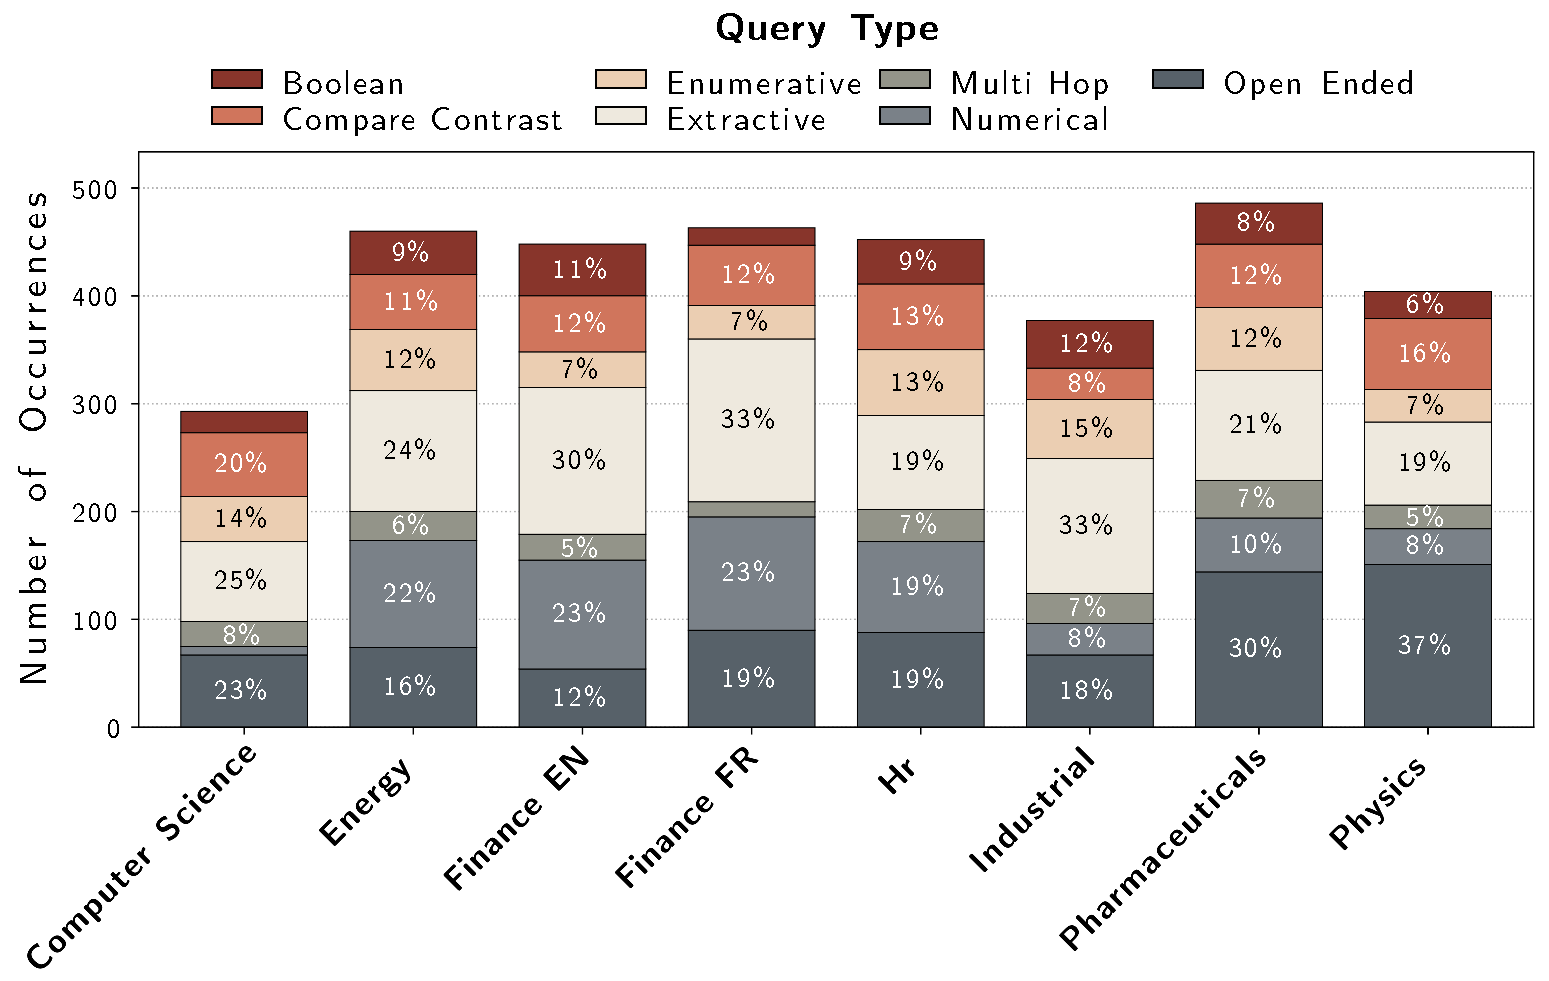
\includegraphics[width=\columnwidth]{images/vidorev3_images/vidore_distribution_acl_v2.pdf}
    \caption{\textbf{Query Type Distribution per Domain}} 
    \label{fig:query_type_distribution}
\end{figure}

\begin{figure}[ht]
    \centering
    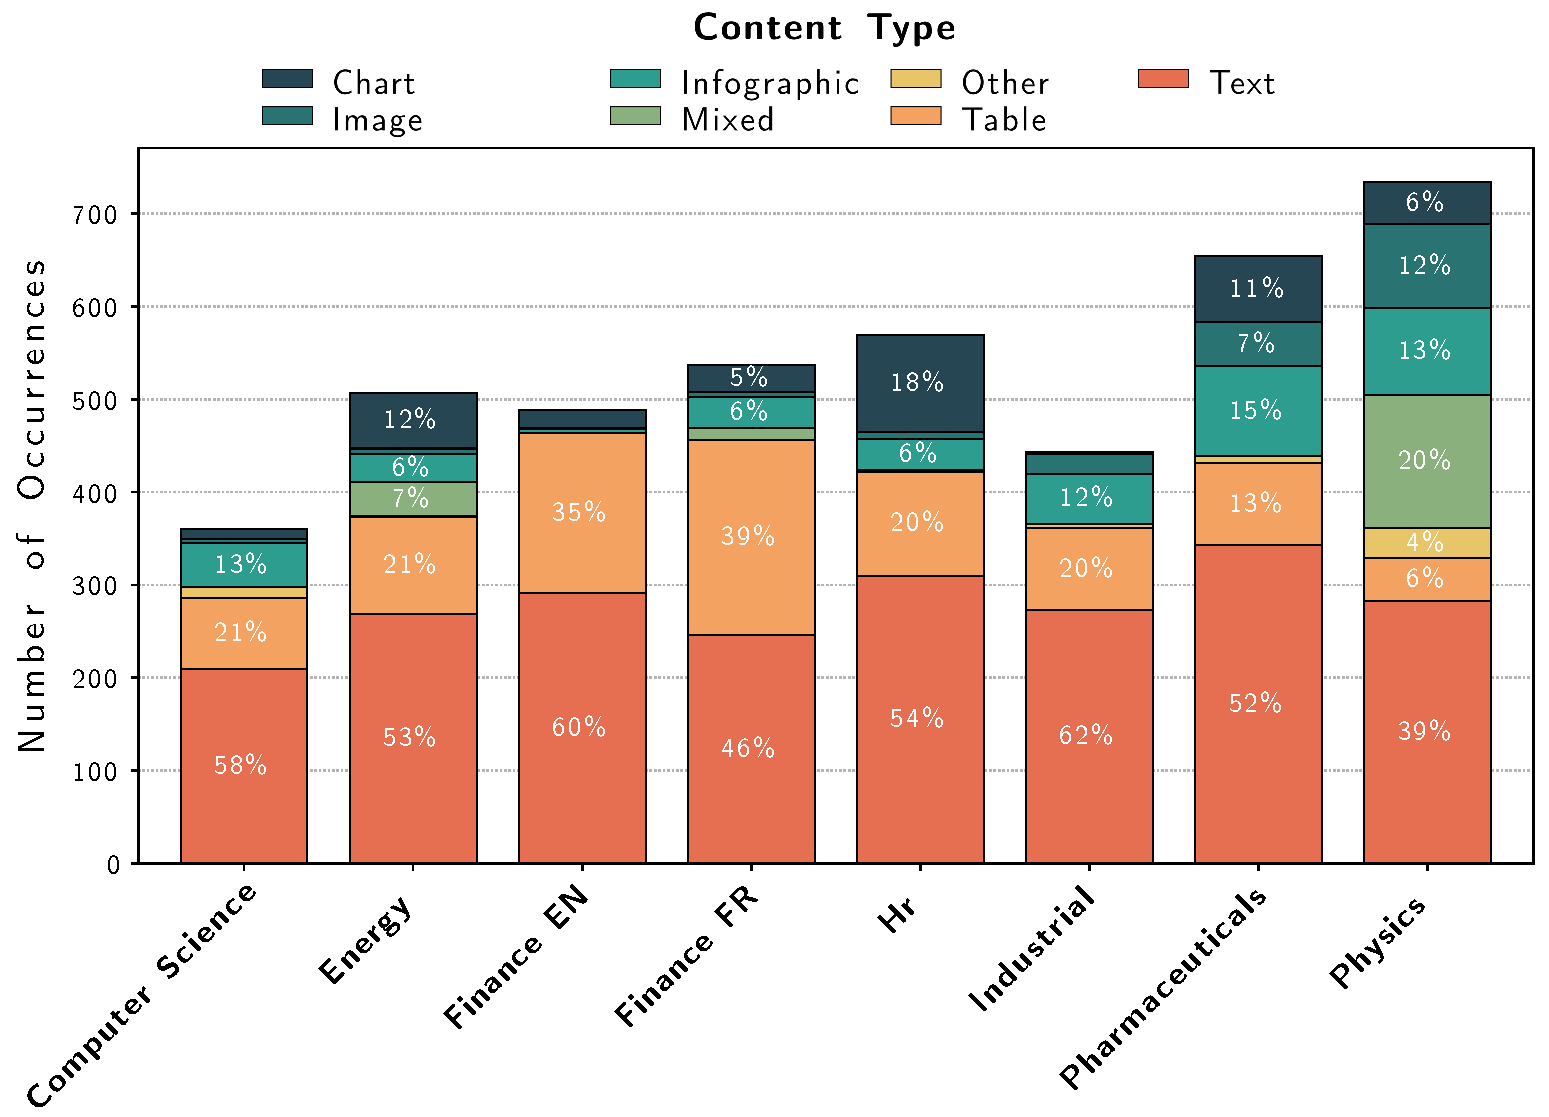
\includegraphics[width=\columnwidth]{images/vidorev3_images/content_type_distribution_acl_v2.pdf}
    \caption{\textbf{Content Type Distribution per Domain}} 
    \label{fig:content_type_distribution}
\end{figure}

% \subsection{Human Annotation}

% \manu{the structure is weird. you mention all the rest and already mention annotators but then have this subsection now. I would perhaps do this the other way around. First put forward human annotators as a jey oart of the pipeline (first thing so it primes readers into trusting the quality), and then detail the various phases. As I mentionned before, I beliebve the entire human in the loop process is a novelty and enables us to produce high qualitry large scale annotations which is not possible without both vompoinents, AI and humns. This could be touched on first, and then detailed. }

%The benchmark was constructed through a two-stage human annotation process designed to produce high-quality queries and reliable ground truth. 

%\paragraph{Annotation Tasks.} The annotation pipeline consisted of two core tasks \gmor{Could you identify in the main figure what are Tasks 1 and Task 2 and reference the image here?}. In the first task, \textit{Query Writing}, annotators reviewed document content and authored queries according to a predefined taxonomy comprising 7 query types and 3 query formats, as detailed in Table~\ref{tab:query_taxonomy}. In the second task, \textit{Query-Page Linking}, annotators performed a comprehensive evaluation: they assessed query quality, rated page relevance on a three-point scale (Not Relevant, Critically Relevant, Fully Relevant), annotated content modalities (Text, Table, Chart, Infographic, Image, or Other), drew bounding boxes around relevant regions, and composed answers to each query. \anto{repeated with 2.3 but better written}


% \paragraph{Annotator Pool and Selection.} Annotation was conducted by a curated pool of 76 annotators who were selected based on having: (1) a bachelor's degree or higher in the relevant domain, (2) professional experience in the domain, (3) native-level language proficiency as required by task, and (4) prior experience with RAG, retrieval, or VQA annotation projects. Quality control was performed by 13 senior annotators with enhanced domain knowledge and extensive annotation experience, with project oversight provided by data leads with multiple years of experience in human data generation. \anto{summarize to one sentence and move the details to appendix}

% \paragraph{Training and Pilot Phase.} The annotation process began with a comprehensive onboarding phase where annotators received task-specific training using gold-standard examples. For each domain, a pilot of several hundred tasks was conducted with 100\% quality control coverage and multiple annotators per task. During this phase, data leads and the research team continuously evaluated annotations, provided clarifications, and refined guidelines. Inter-annotator agreement and time-per-task baselines were calculated to establish ongoing evaluation benchmarks. The pilot concluded upon validation of both data quality and guideline effectiveness. \anto{Move this to appendix}



% \paragraph{Inter-Annotator Agreement.} \anto{We can shorten this and just say that we use Gwet’s AC2 because it's stable under prevalence skew and Weighted Agreement} Because pages were pre-filtered by a VLM before human annotation, most pages shown to annotators were likely relevant, creating a skewed class distribution. This prevalence imbalance causes traditional chance-corrected metrics like Krippendorff's Alpha to appear paradoxically low even when annotators genuinely agree, as inflated expected chance agreement penalizes the score. To address this, we report 3 complementary metrics: Krippendorff's Alpha (ordinal) as the standard measure, Gwet's AC2 which remains stable under prevalence skew, and Weighted Agreement as a raw consistency measure. Overall, annotators achieved $\alpha = 0.469$, AC2 $= 0.760$, and Weighted Agreement $= 0.815$. The divergence between Alpha and AC2/Weighted Agreement is expected given the pre-filtered data and confirms substantial agreement despite the skewed distribution.

\subsection{Dataset Release and Distribution}

%Reflecting the reality of globalized enterprises where knowledge bases are often monolingual while the workforce is distributed\vic{remove this},
We extend the benchmark to rigorously assess cross-lingual retrieval. While source documents are maintained in English and French, we use Qwen3-235B-Instruct to provide translations in 6 languages: English, French, Spanish, German, Italian, and Portuguese. This configuration challenges models to bridge the semantic gap between the query language and the document language, a critical requirement for modern RAG systems. 

Finally, to ensure the integrity of evaluation and mitigate data contamination (which was shown to be a major preoccupation for Information Retrieval \sidecite{rteb2025}), we adopt a split-release strategy. 8 datasets are made public to facilitate research, while 2 are retained as private hold-out sets. This enables blind evaluation, ensuring that performance metrics reflect true generalization rather than overfitting to public samples.

%Finally, to ensure the integrity of evaluation and mitigate data contamination (which was shown to be a major preoccupation for Information Retrieval \sidecite{rteb2025}), we adopt a split-release strategy. 8 datasets are made public to facilitate research, while 2 are retained as private hold-out sets. This enables blind evaluation via the MTEB leaderboard, ensuring that performance metrics reflect true generalization rather than overfitting to public samples.

% \subsection{Cross-Lingual Extension} \vic{TODO Quentin combine with following subsection}.

% Real-world enterprise knowledge bases are often dominated by English or dominant local languages, while the workforce can be globally distributed. To assess cross-lingual retrieval capabilities, the benchmark includes source documents in both English and French, paired with queries in 6 different languages ({English, French, Spanish, German, Italian, and Portuguese}). This setup challenges models to bridge the semantic gap between the query language and the document language, a critical requirement for globalized RAG systems.

% \subsection{Benchmark Splitting}

% To ensure the integrity of evaluation and prevent data contamination (which was shown to have a significant impact on IR evaluation \que{CITE MTEB v2}), we adopt a split-release strategy. 8 datasets are publicly released to facilitate research and model development, while two datasets are retained as private hold-out sets. \anto{Which ones?} This design allows for a robust, blind evaluation on the MTEB leaderboard, ensuring that high performance reflects genuine generalization capabilities rather than overfitting to public data distributions.

% \begin{figure*}[H]
%     \centering
%     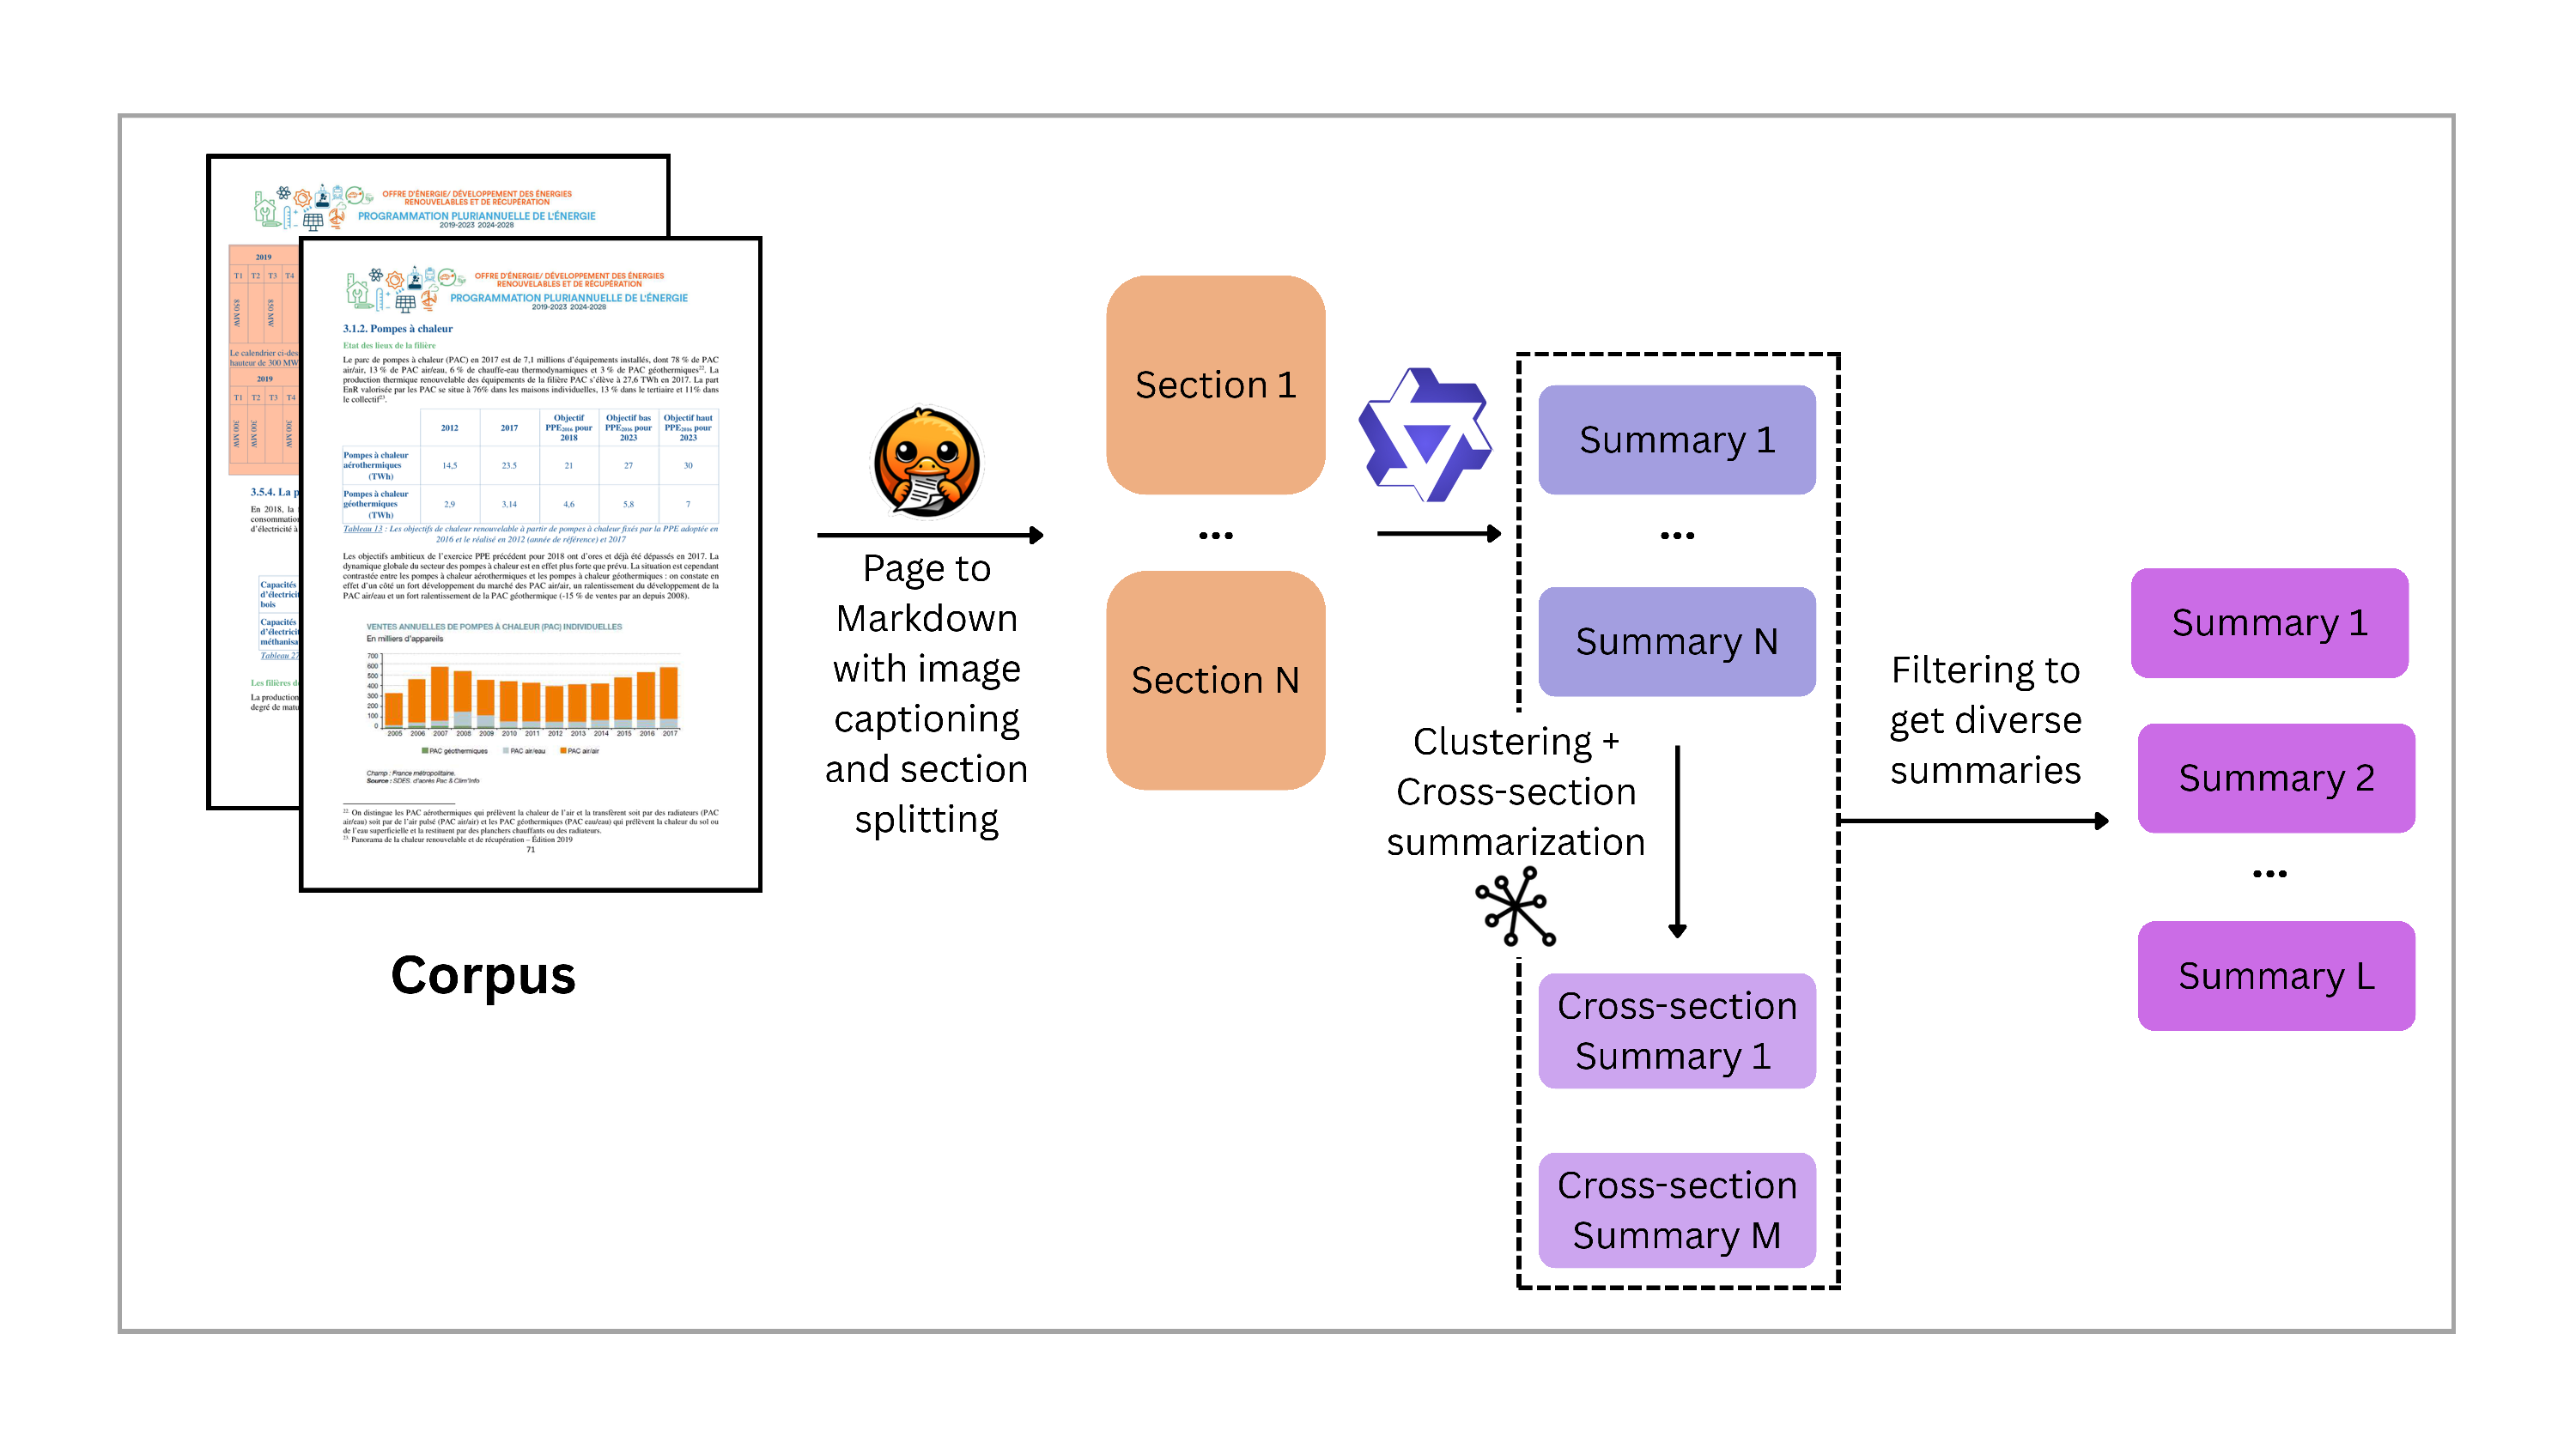
\includegraphics[trim={0cm 2cm 0cm 2cm}, clip, width=\textwidth]{images/vidorev3_images/summary_generation.pdf}
%     \caption{Summarization Process}
%     \label{fig:lf_architecture}
% \end{figure*}

% \begin{figure*}[H]
%     \centering
%     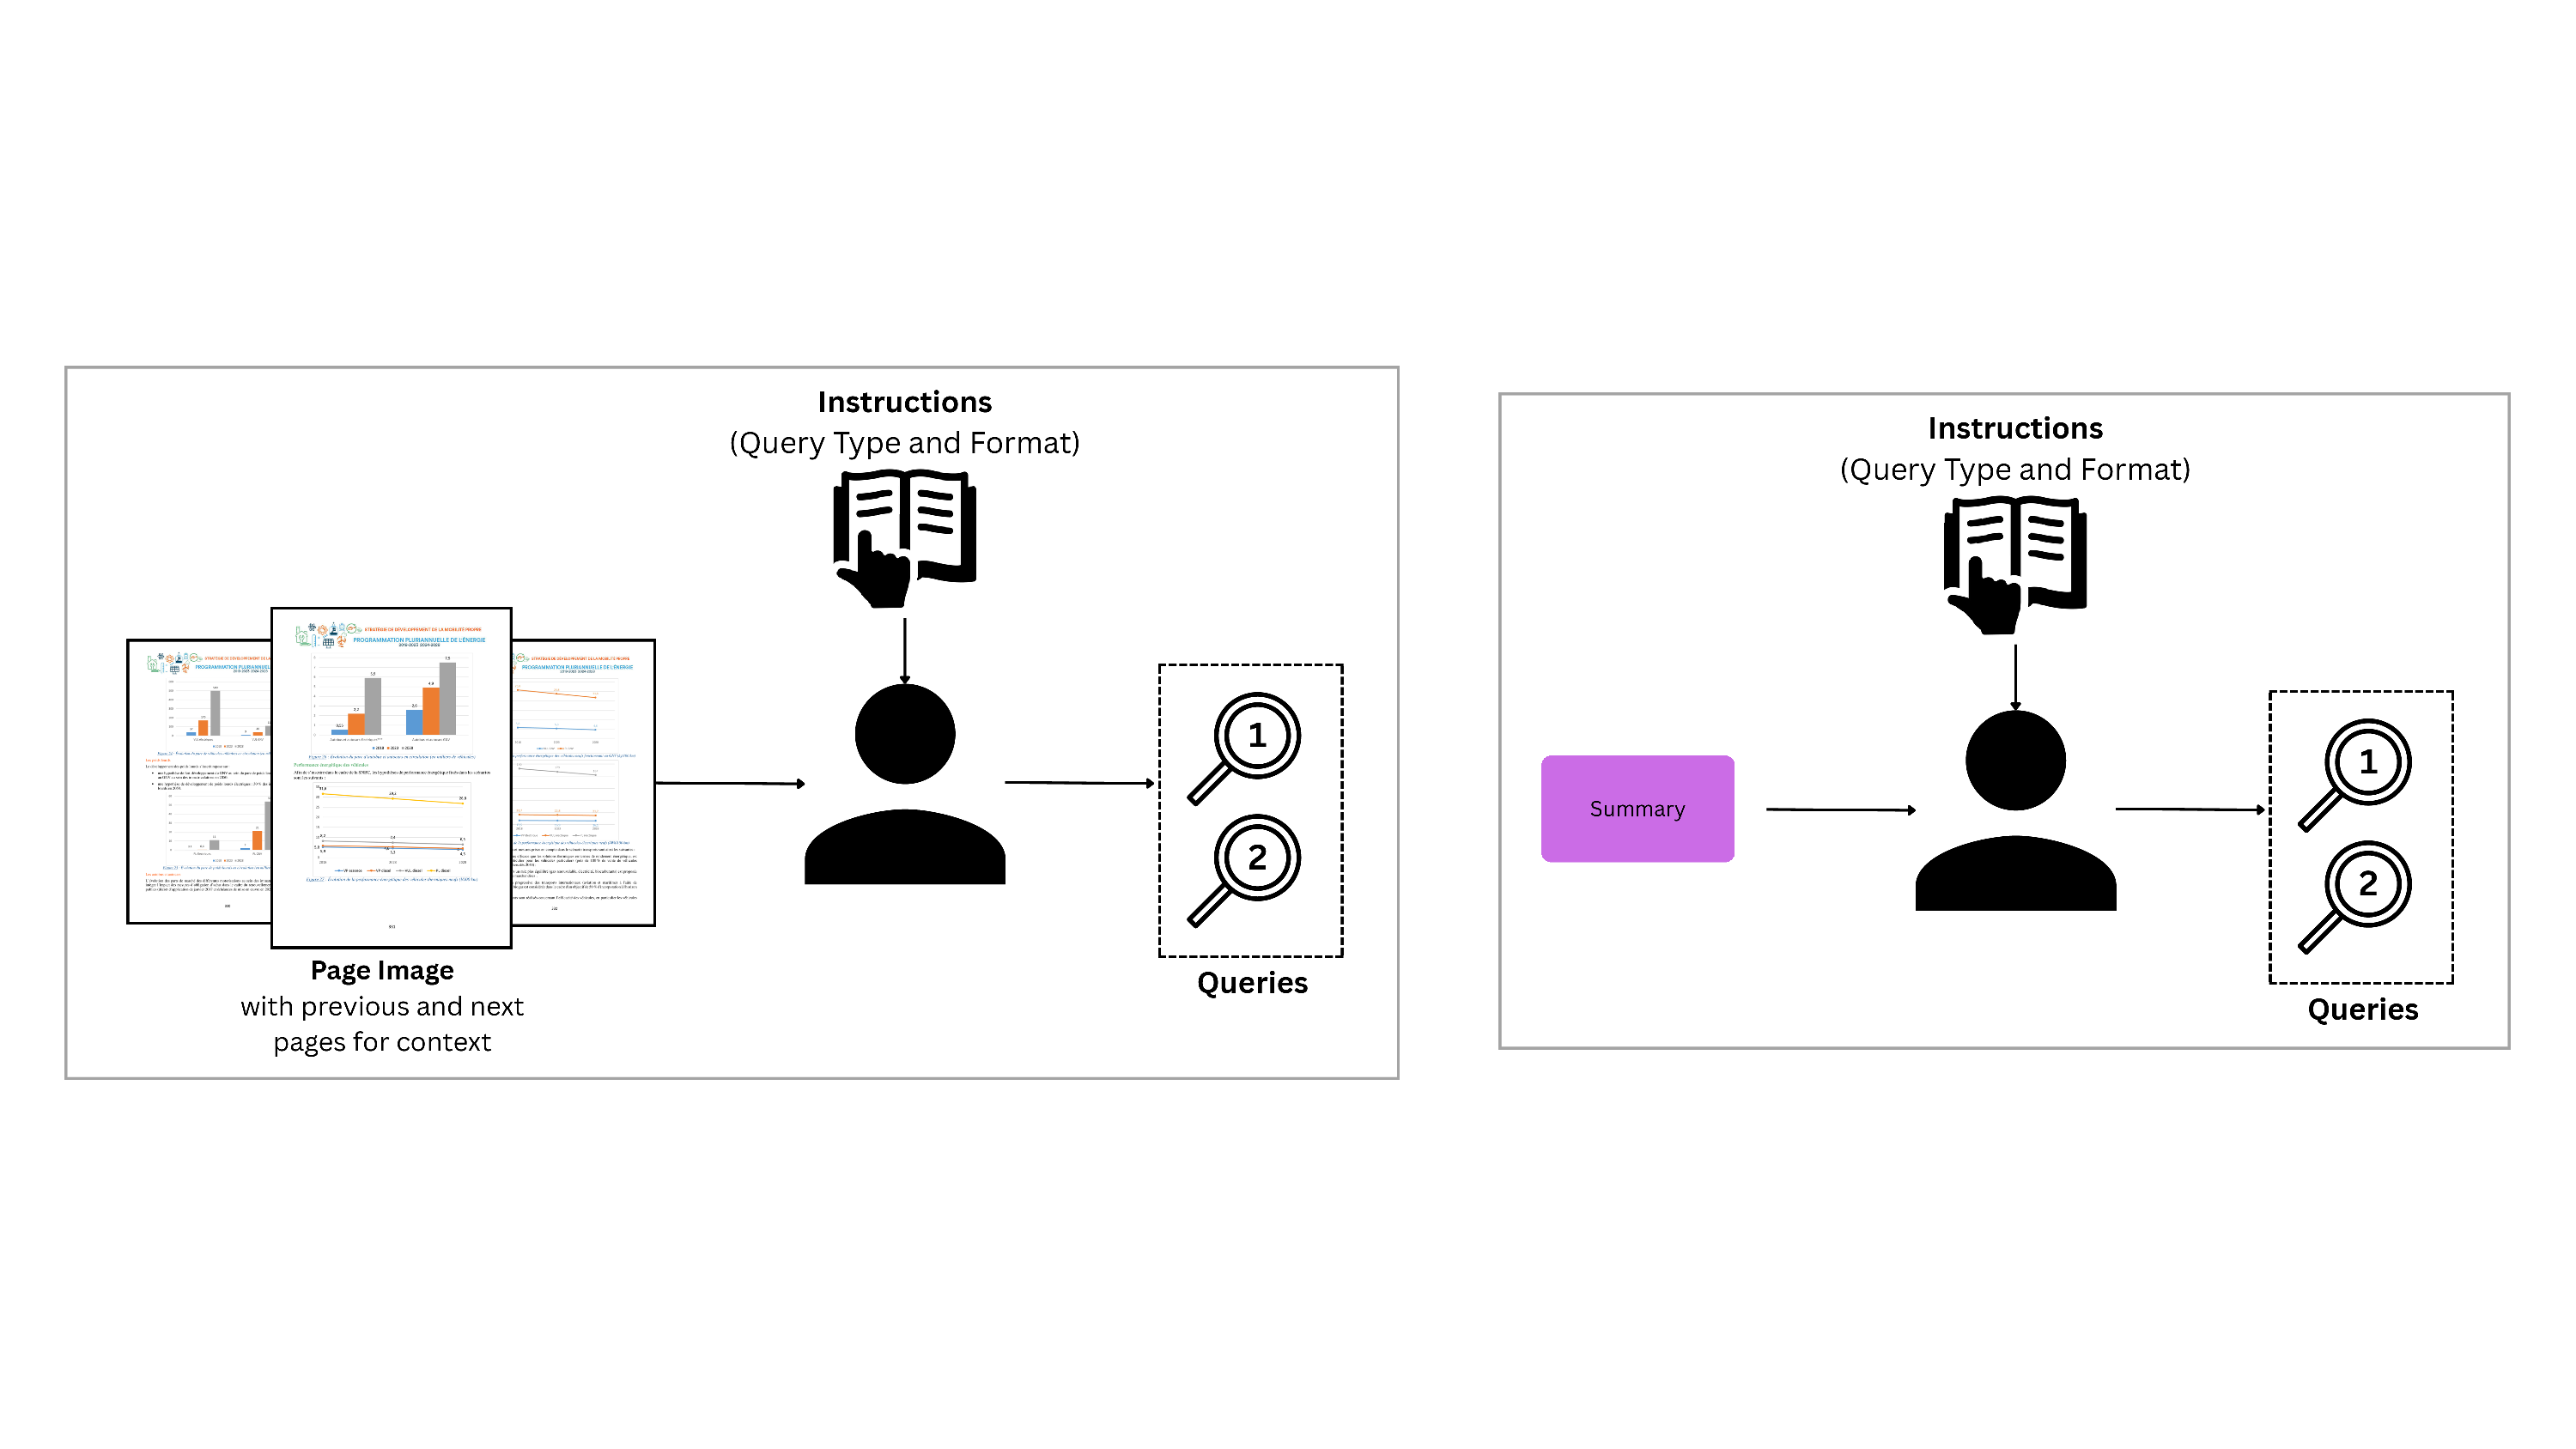
\includegraphics[trim={0cm 7cm 0cm 6cm}, clip, width=\textwidth]{images/vidorev3_images/human_query_generation.pdf}
%     \caption{Human Query Generation Process}
%     \label{fig:query_page_linking}
% \end{figure*}

% \begin{figure*}[H]
%     \centering
%     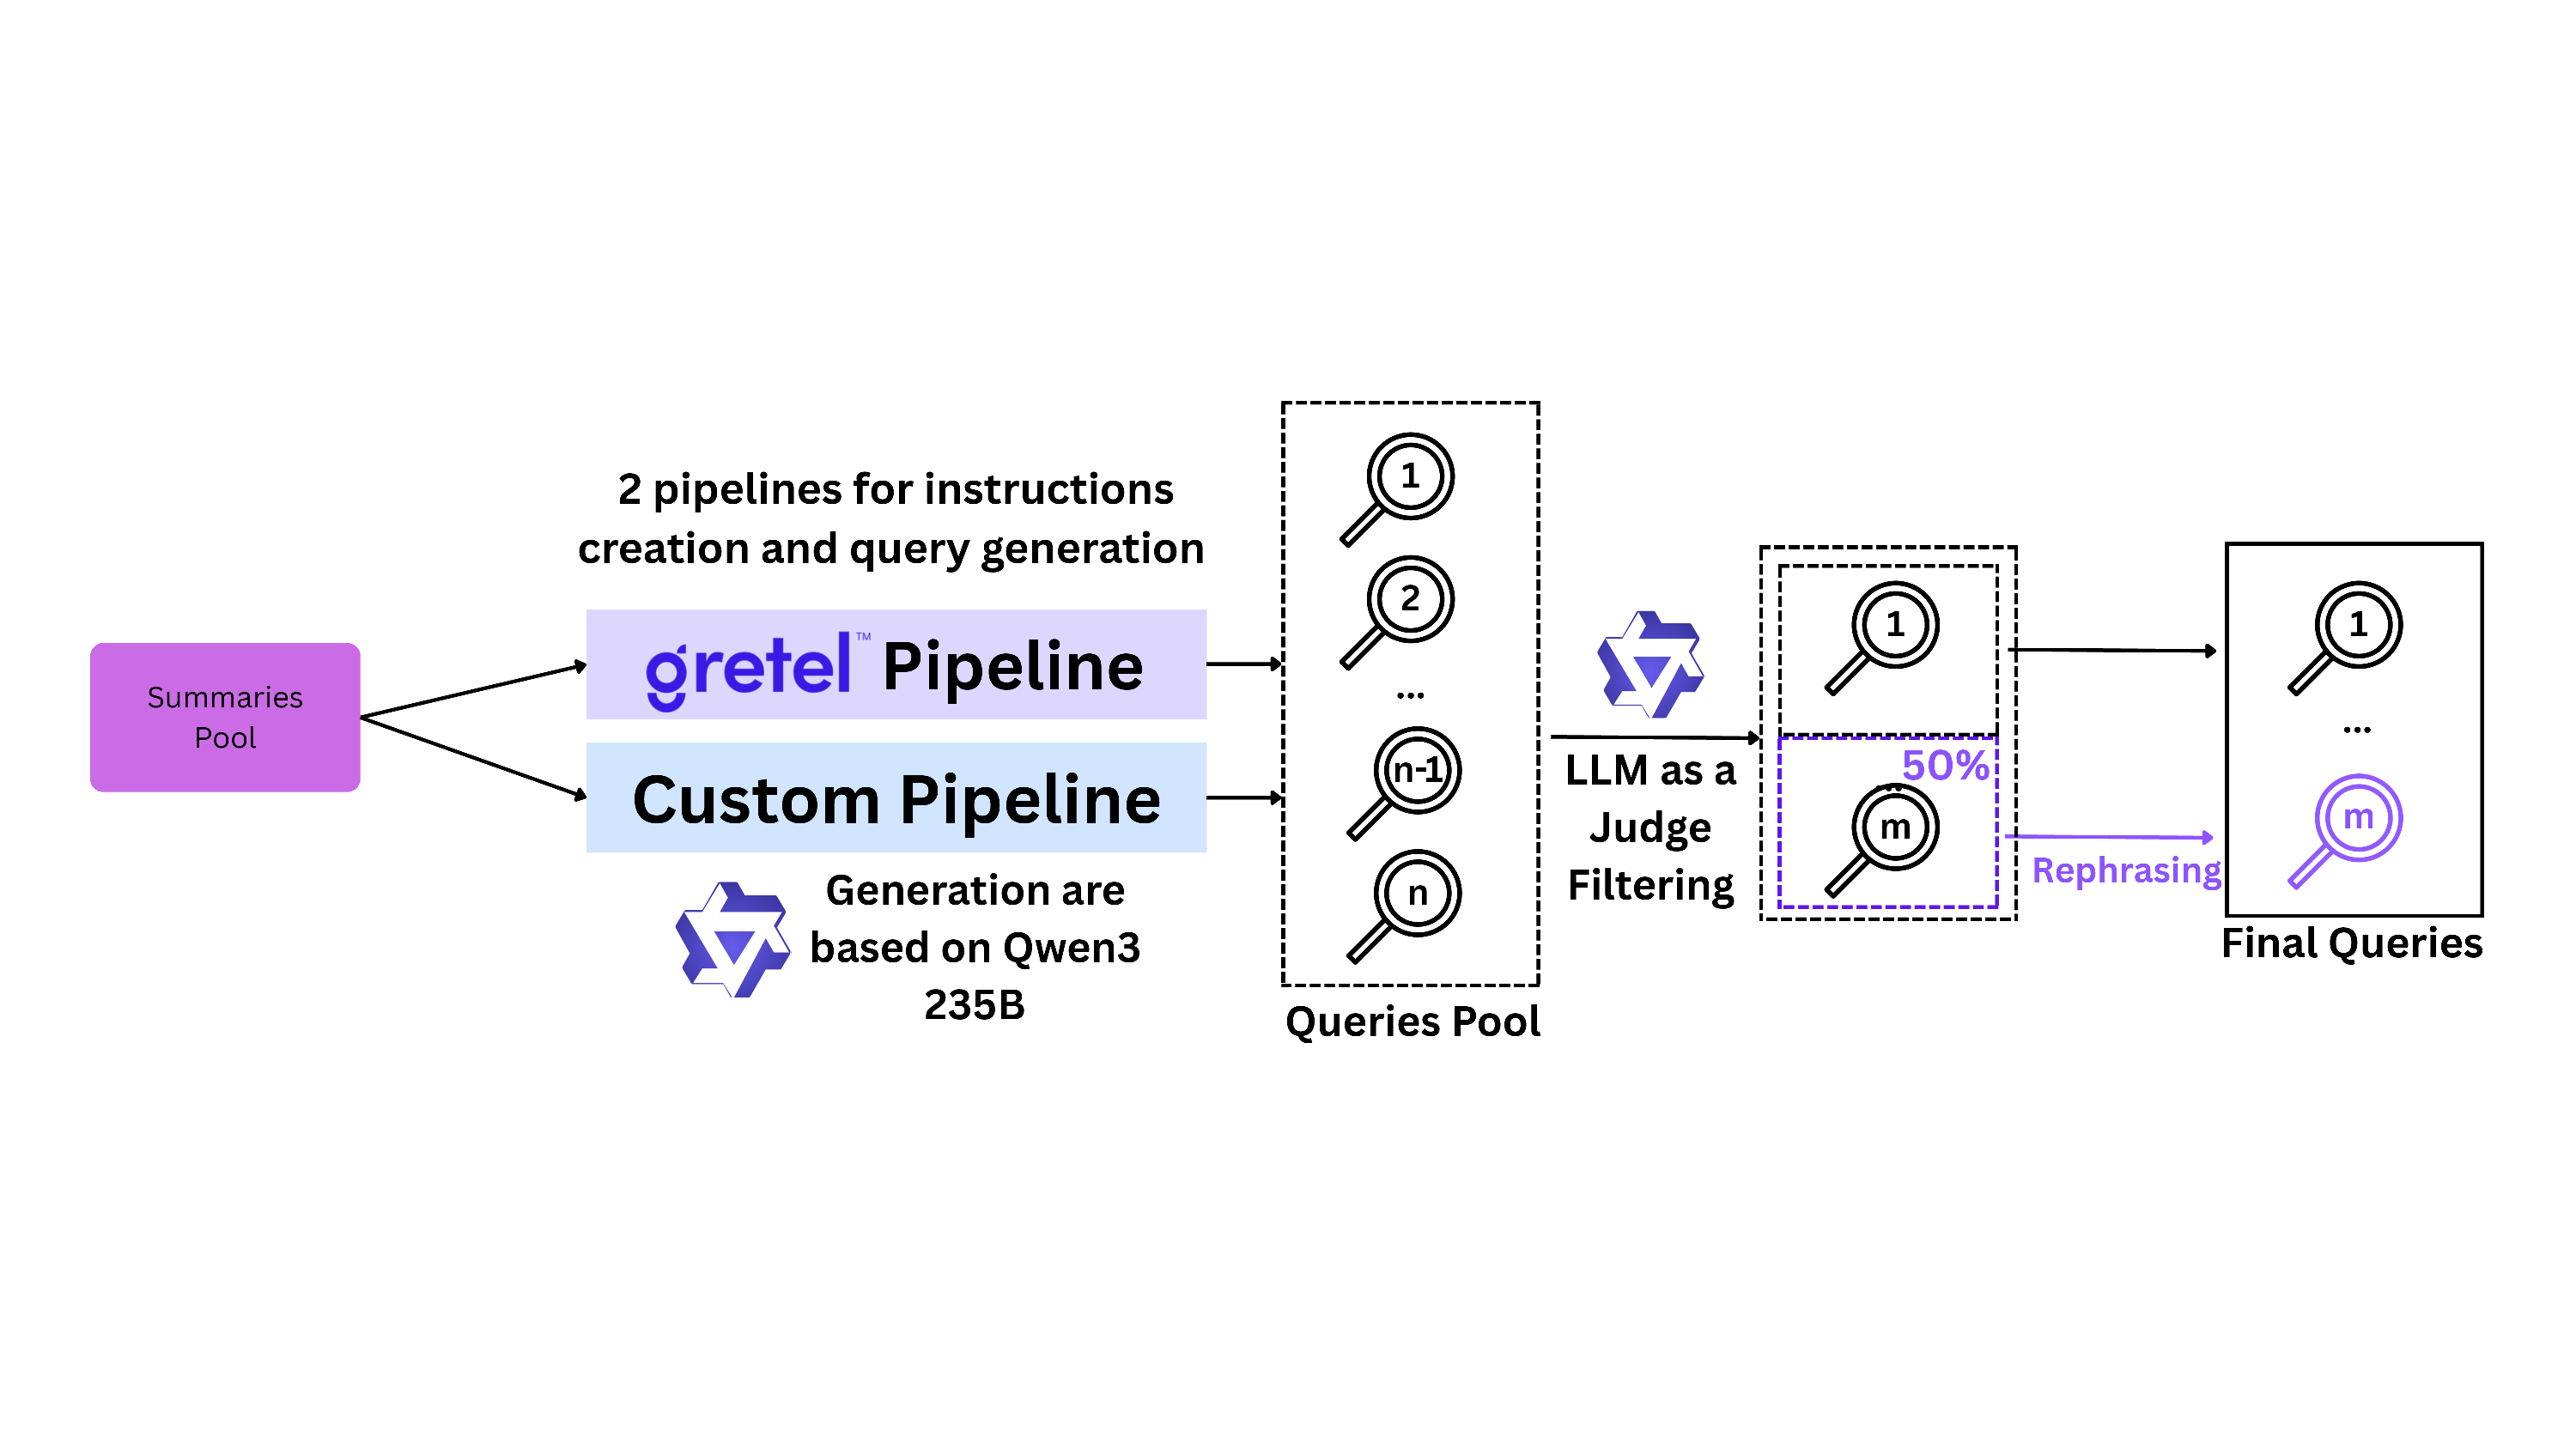
\includegraphics[trim={0cm 7cm 0cm 7cm}, clip, width=\textwidth]{images/vidorev3_images/synthetic_query_generation.pdf}
%     \caption{Synthetic Query Generation Process}
%     \label{fig:query_page_linking}
% \end{figure*}

% \begin{figure*}[H]
%     \centering
%     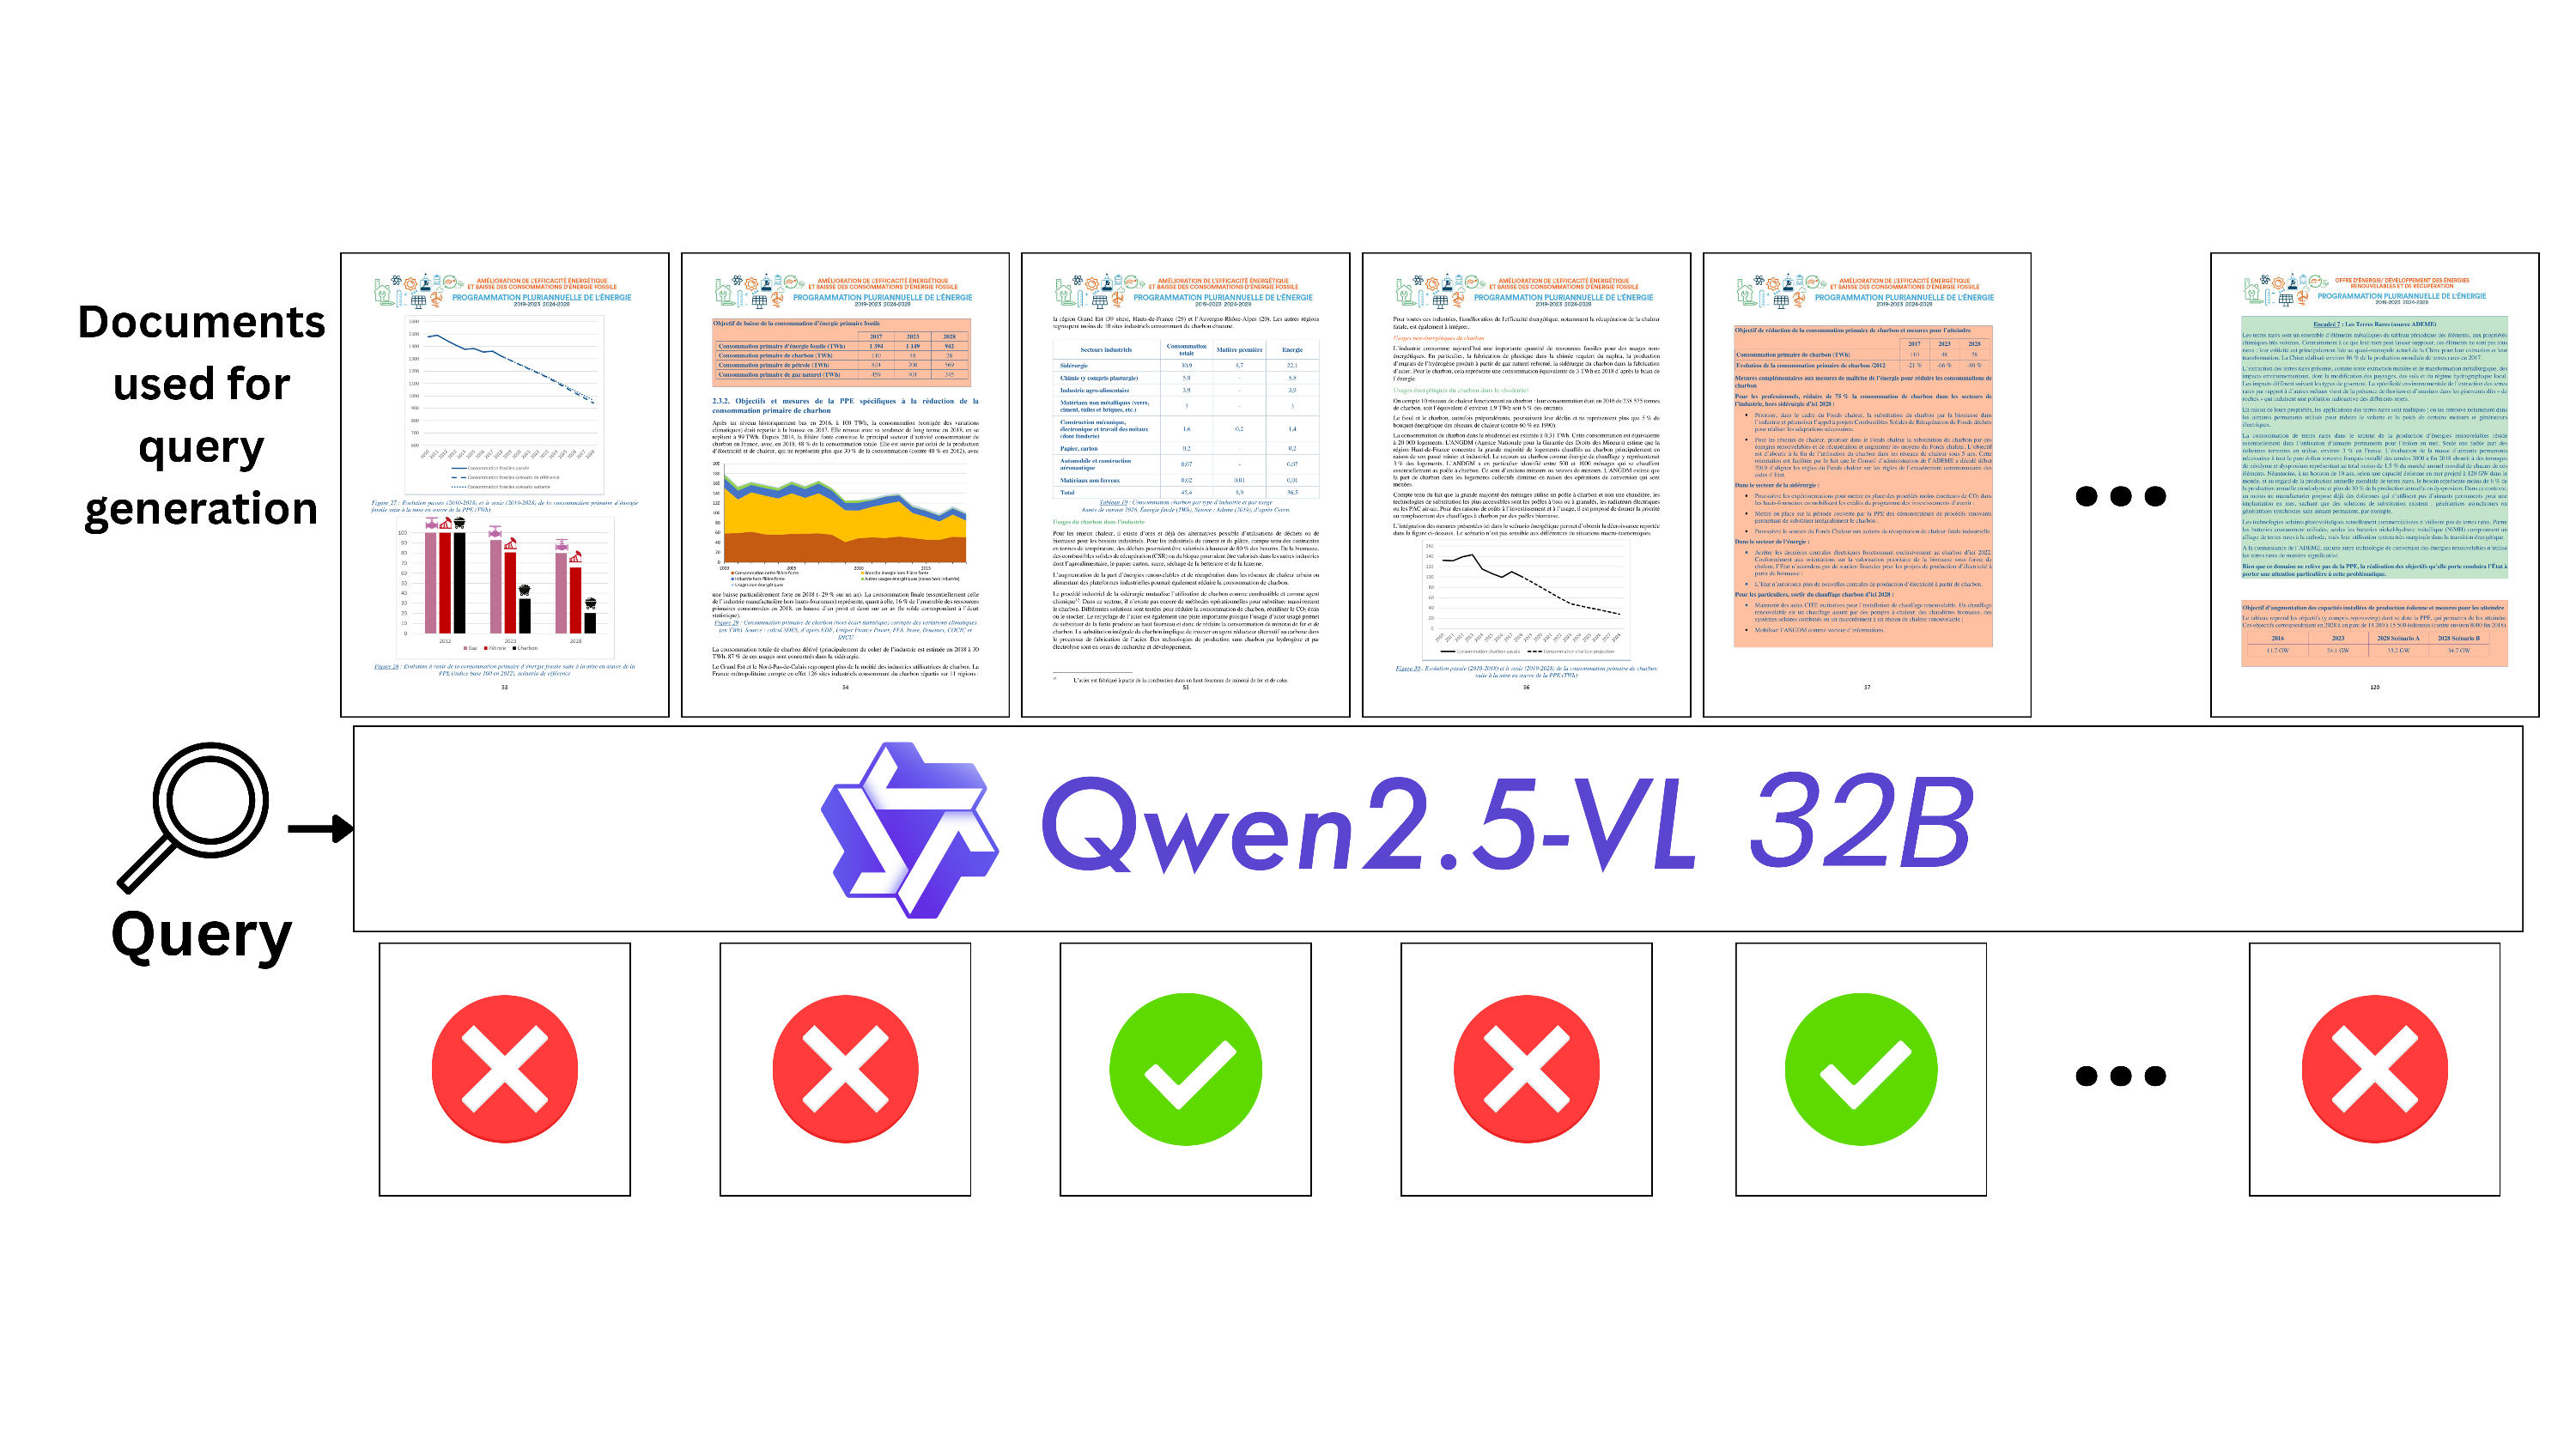
\includegraphics[trim={0cm 4cm 0cm 3cm}, clip, width=\textwidth]{images/vidorev3_images/query_page_linking.pdf}
%     \caption{Query Page Linking Process}
%     \label{fig:query_page_linking}
% \end{figure*}

\section{Experiments and Results}

Using our benchmark, we conduct extensive evaluations across all 3 components of RAG pipelines. We assess textual and visual retrievers and rerankers on retrieval performance, evaluate leading VLMs and LLMs on their ability to generate accurate answers from various retrieved contexts, and test VLMs on bounding box generation for visual grounding. From these results, we compile practical insights for RAG practitioners.

% \begin{figure}[H]
%     \centering
%     \includegraphics{images/vidorev3_images/human_vs_sdg.pdf}
%     \caption{Performance of ColQwen2.5 on human VS SDG queries generated from summaries}
%     \label{fig:lf_architecture}
% \end{figure}

% \begin{figure}[H]
%     \centering
%     \includegraphics{images/vidorev3_images/human_sum_vs_human_img.pdf}
%     \caption{Performance of ColQwen2.5 on human queries from summaries VS human queries from images}
%     \label{fig:lf_architecture}
% \end{figure}

% \begin{figure}[H]
%     \centering
%     \includegraphics{images/vidorev3_images/custom_gretel_human.pdf}
%     \caption{Human preference between custom pipeline, Gretel pipeline and human queries according to several criteria}
%     \label{fig:lf_architecture}
% \end{figure}

\begin{table*}[h!]
\small
\centering
\resizebox{\textwidth}{!}{%
\begin{tabular}{l c c c c c c c c c c c >{\columncolor{avgcol}}c}
\toprule
 & & \multicolumn{7}{c}{\textbf{English Datasets}} & \multicolumn{3}{c}{\textbf{French Datasets}} & \multicolumn{1}{c}{} \\
\cmidrule(lr){3-9} \cmidrule(lr){10-12}
\textbf{Model} & Size (B) & \shortstack{C.S.} & \shortstack{Nucl.} & \shortstack{Fin.} & \shortstack{Phar.} & \shortstack{H.R.} & \shortstack{Ind.} & \shortstack{Tel.} & \shortstack{Phys.} & \shortstack{Ener.} & \shortstack{Fin.} & \textbf{Avg.} \\
\midrule
\multicolumn{13}{l}{\textit{\textbf{Textual Retrievers}}} \\
Qwen3-8B$^\bigstar$  & 8 & \textbf{71.7} & 39.0 & \textbf{49.4} & \textbf{59.2} & 47.6 & \textbf{40.4} & \textbf{62.8} & \textbf{45.6} & 58.9 & 35.8 & \textbf{51.0} \\
Jina-v4 & 3 & 64.3 & \textbf{44.3} & 48.4 & 54.9 & \textbf{52.8} & 38.4 & 56.3 & 43.6 & \textbf{60.1} & \textbf{41.3} & 50.4 \\
LFM2-350M & 0.35 & 63.5 & 37.8 & 39.0 & 56.4 & 43.5 & 34.4 & 56.9 & 41.8 & 47.0 & 28.2 & 44.9 \\
Qwen3-0.6B$^\bigstar$  & 0.6 & 66.4 & 32.8 & 42.7 & 50.6 & 37.7 & 31.6 & 55.7 & 43.3 & 51.3 & 25.8 & 43.8 \\
BGE-M3$^\bigstar$  & 0.57 & 58.0 & 30.2 & 39.8 & 52.0 & 42.4 & 28.5 & 51.6 & 35.9 & 49.8 & 25.2 & 41.3 \\
BM25S & - & 28.7 & 17.4 & 17.6 & 27.3 & 12.8 & 15.6 & 33.3 & 14.8 & 21.9 & 14.0 & 20.3 \\
\midrule
\multicolumn{13}{l}{\textit{\textbf{Visual Retrievers}}} \\
%tomoro-colqwen3-8b$^\blacktriangle$ & 8 & 75.4 & \textbf{52.7} & \textbf{65.1} & \textbf{66.4} & \textbf{64.0} & \textbf{54.4} & \textbf{70.5} & \textbf{50.1} & \textbf{68.4} & \textbf{49.1} & \textbf{61.6}\\
%tomoro-colqwen3-4b$^\blacktriangle$ & 4 & 75.5 & 51.2 & 63.8 & 65.7 & 60.1 & 53.6 & 69.4 & 48.3 & 66.4 & 46.8 & 60.2\\
ColEmbed-3B-v2 & 3 & \textbf{77.1} & \textbf{50.7} & \textbf{64.2 }& \textbf{66.0} & \textbf{62.3} & \textbf{51.7} & \textbf{69.7} & 47.0 & 64.9 & 44.4 & \textbf{59.8} \\
Jina-v4 & 3 & 71.8 & 50.0 & 59.3 & 63.1 & 59.5 & 50.4 & 64.8 & 46.6 & 64.0 & \textbf{46.1} & 57.6 \\
ColNomic-7B & 7 & 76.2 & 45.0 & 56.6 & 62.3 & 58.7 & 50.1 & 67.2 & \textbf{48.3} & 64.0 & 45.5 & 57.4 \\
ColEmbed-3B & 3 & 75.2 & 49.1 & 60.9 & 63.7 & 58.7 & 47.1 & 67.0 & 45.1 & 62.1 & 43.8 & 57.3 \\
ColNomic-3B & 3 & 72.7 & 42.1 & 56.3 & 61.1 & 57.3 & 47.4 & 64.5 & 47.5 & \textbf{65.0} & 44.3 & 55.8 \\
ColEmbed-1B & 1 & 71.3 & 47.3 & 58.9 & 62.6 & 57.0 & 46.6 & 64.7 & 44.1 & 60.9 & 42.4 & 55.6 \\
ColQwen2.5 & 3 & 72.3 & 38.1 & 52.3 & 57.9 & 51.2 & 41.3 & 61.3 & 45.9 & 59.7 & 39.1 & 51.9 \\
Nomic-7B$^\bigstar$  & 7 & 66.6 & 36.7 & 48.8 & 58.9 & 46.2 & 37.9 & 57.8 & 44.2 & 57.5 & 36.0 & 49.0 \\
ColQwen2 & 2 & 68.6 & 35.7 & 39.0 & 52.2 & 45.1 & 38.3 & 57.4 & 41.6 & 48.8 & 20.0 & 44.7 \\
Nomic-3B$^\bigstar$ & 3 & 58.5 & 32.2 & 44.2 & 55.3 & 43.3 & 33.2 & 53.7 & 42.0 & 51.4 & 28.9 & 44.3 \\
ColPali & 7 & 65.3 & 32.9 & 34.4 & 53.1 & 44.8 & 35.6 & 54.0 & 41.7 & 47.1 & 21.8 & 43.1 \\
\bottomrule
\end{tabular}
}
\caption{\textbf{Retrieval performance (NDCG@10) across the benchmark.} Best results per category in bold. \mbox{$\bigstar$: single-vector models}. Following MTEB conventions, the average score is a macro-average over all datasets. Full model names and references are found in Table~\ref{tab:model_metadata}.} %\boliu{FYI: I updated the full name of ColEmbed-3B-v2 in Table 9, to be consistent to ColEmbed-3B-v1} \anto{thank you}
\label{tab:retriever_comparison_updated}
\end{table*}

\subsection{Retrieval} \label{sec:retrieval results}

We evaluate a large panel of visual and textual retrievers on page-level retrieval ability. Visual retrievers are given page images, while textual retrievers process the Markdown text of each page processed by the NeMo Retriever extraction service\footnote{Chunking within pages or providing image descriptions did not improve our results. Thus, we report the results of the simplest pipeline.} \sidecite{nvidiaocr}. The results reported in Table~\ref{tab:retriever_comparison_updated} corroborate findings from existing document retrieval benchmarks \sidecite{faysse2025colpaliefficientdocumentretrieval,günther2025jinaembeddingsv4universalembeddingsmultimodal}: for a given parameter count, visual retrievers outperform textual retrievers, and late interaction methods score higher than dense methods.



% \begin{figure*}[h]
%     \centering
%     \begin{subfigure}[t]{0.32\textwidth}
%         \centering
%         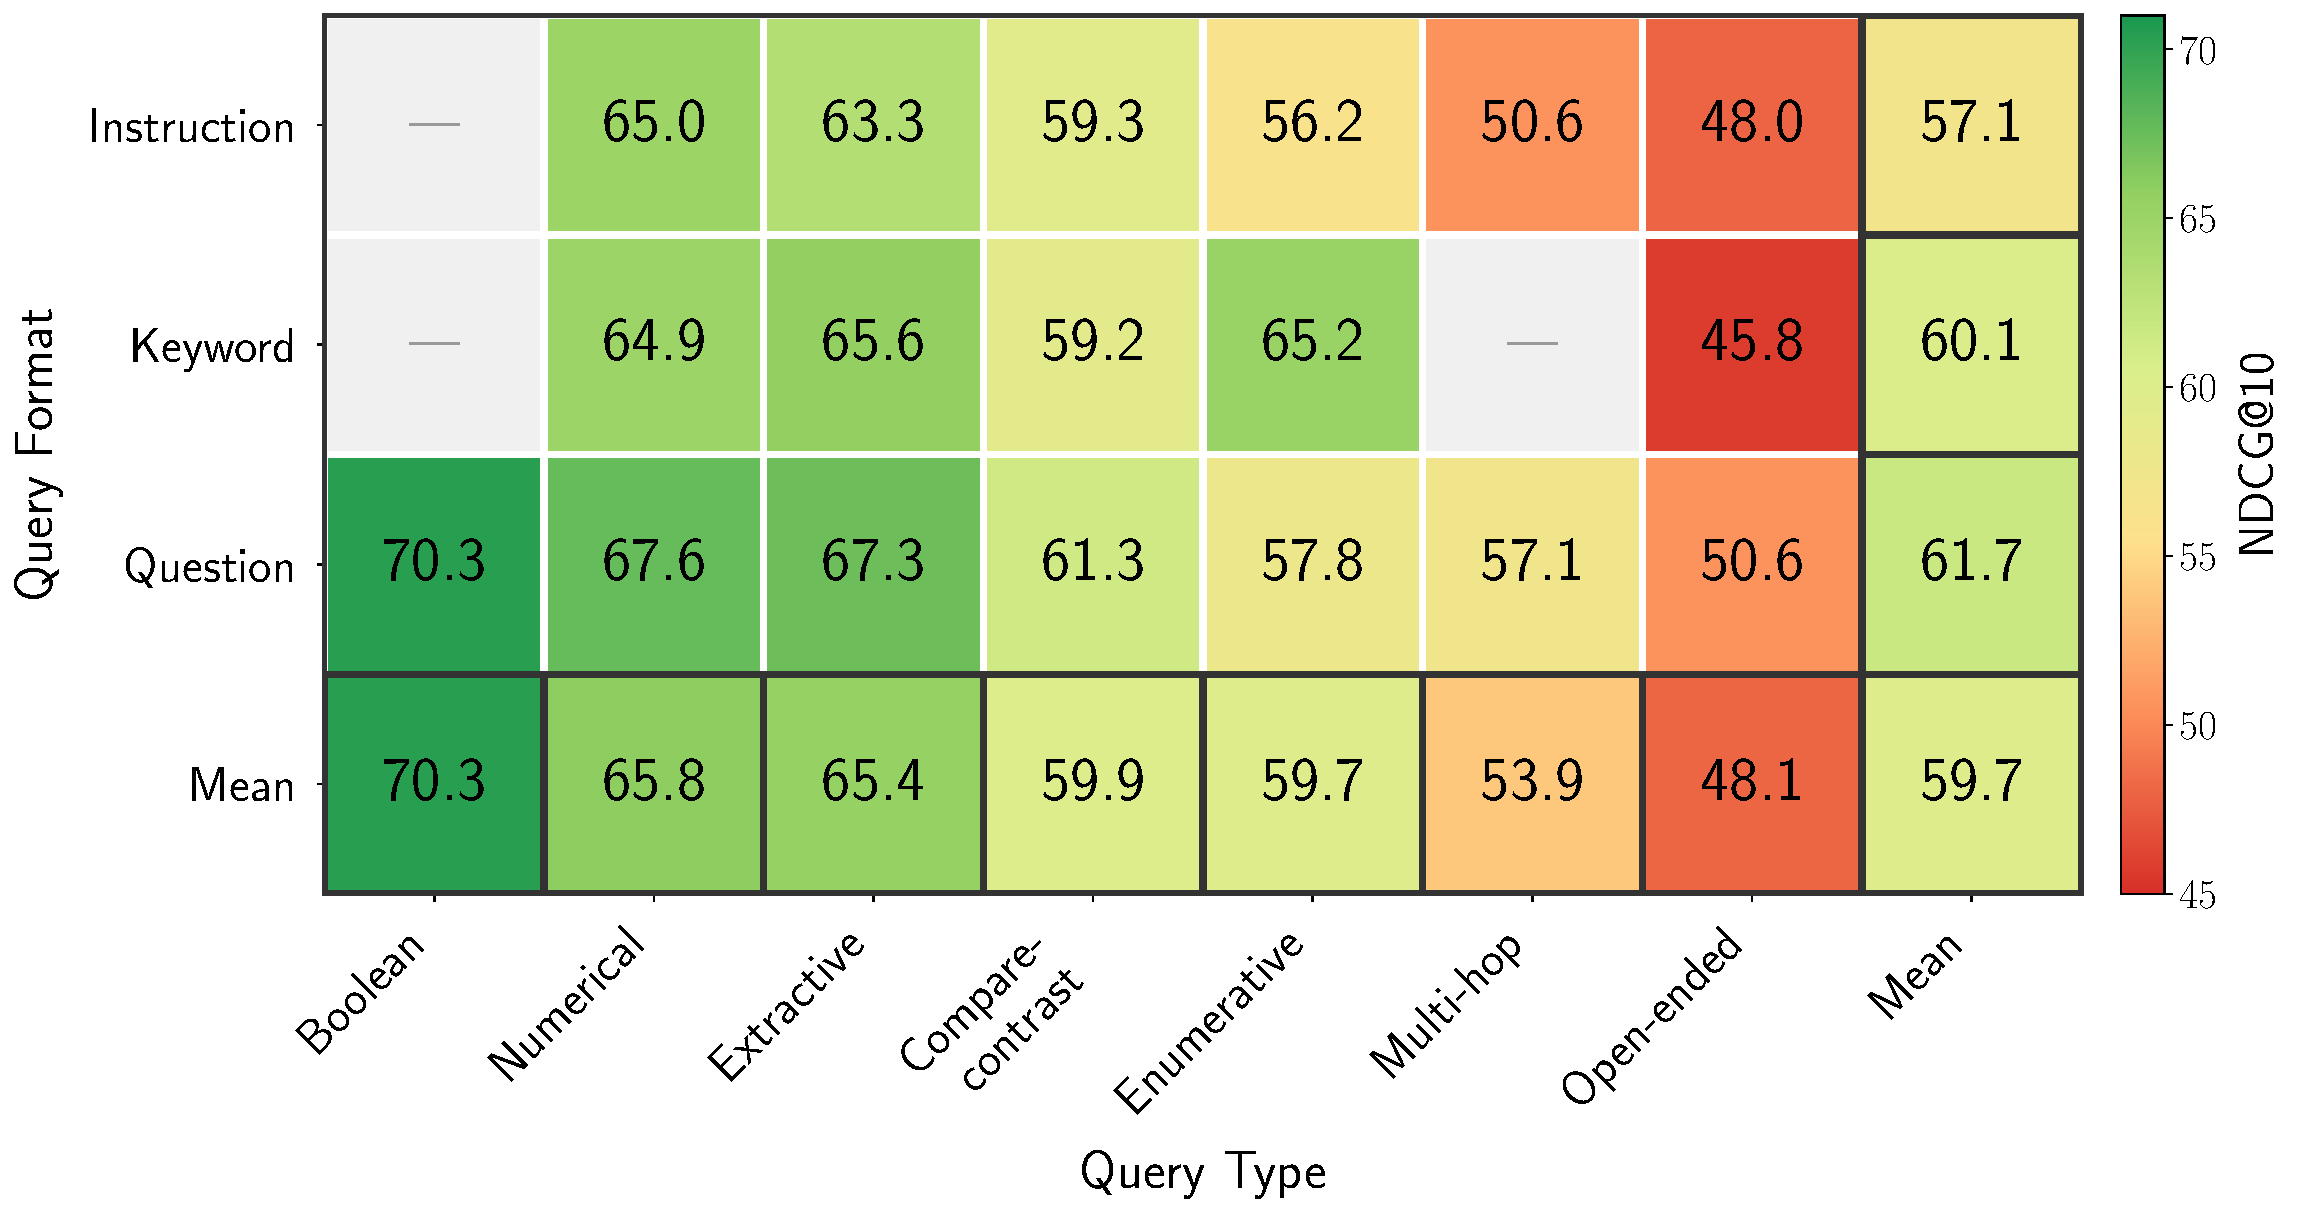
\includegraphics[width=\textwidth]{images/vidorev3_images/ndcg_by_type_format_transposed.pdf}
%         \caption{NDCG@10 by query type and format.}
%         \label{fig:ndcg_type_format}
%     \end{subfigure}
%     \hfill
%     \begin{subfigure}[t]{0.32\textwidth}
%         \centering
%         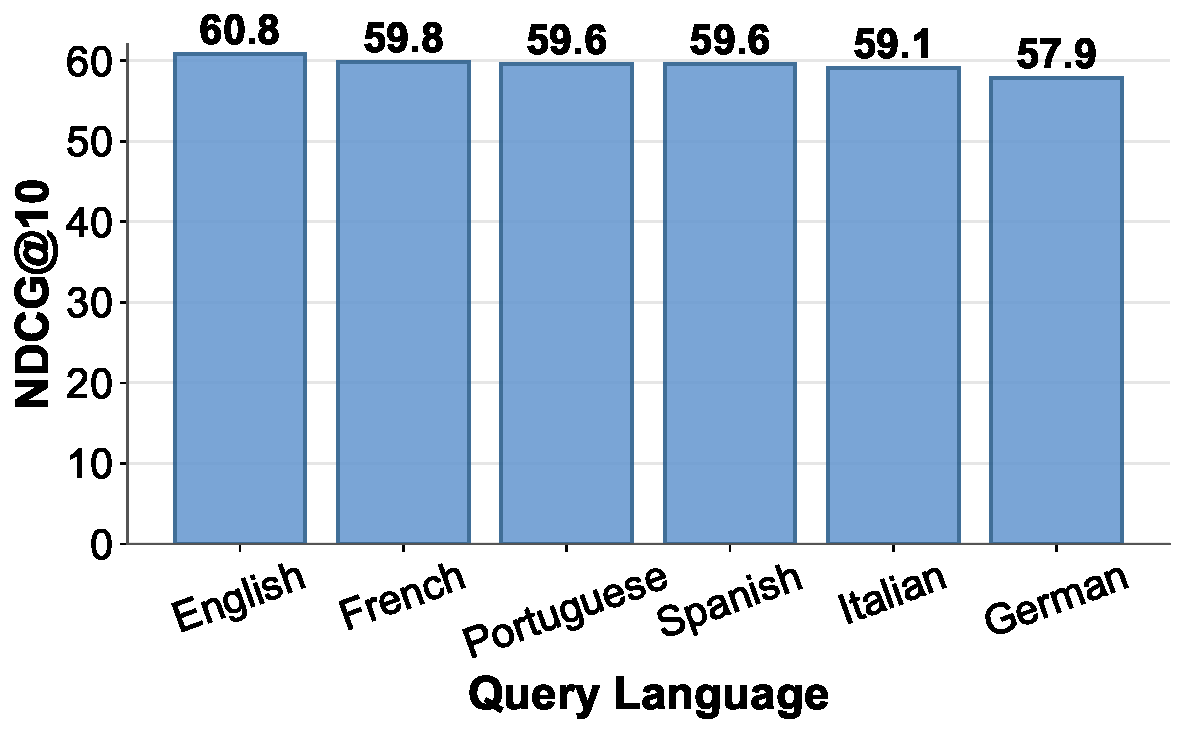
\includegraphics[width=\textwidth]{images/vidorev3_images/ndcg_by_language.pdf}
%         \caption{NDCG@10 by query language.}
%         \label{fig:ndcg_language}
%     \end{subfigure}
%     \hfill
%     \begin{subfigure}[t]{0.32\textwidth}
%         \centering
%         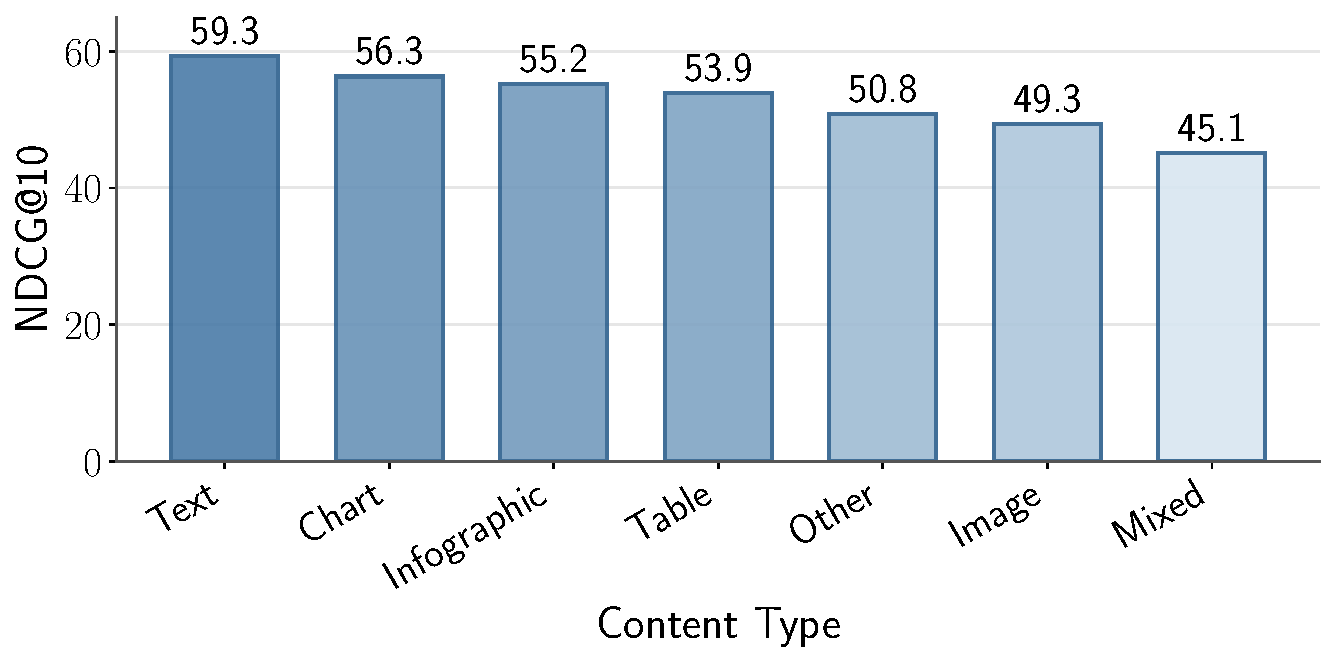
\includegraphics[width=\textwidth]{images/vidorev3_images/ndcg_by_content_type.pdf}
%         \caption{NDCG@10 by content type.}
%         \label{fig:ndcg_content}
%     \end{subfigure}
%     \caption{\textbf{ColEmbed-3B-v2 performance analysis.}}
%     \label{fig:ndcg_analysis}
% \end{figure*}
% je te laisse faire
%on vire the perf of? c'est anglais ? ok
We analyze ColEmbed-3B-v2, the best-performing retriever we evaluated across query type, content modality, and query language. % detailed results are reported in Appendix~\ref{appendix:supp retrieval}.

\paragraph{Performance is aligned with query complexity}
\Cref{fig:type-format-performance} shows that performance is inversely correlated with query complexity: simple query types such as Boolean and Numerical score significantly higher than Open-ended and Multi-hop queries. Question formulations consistently outperform Instruction and Keyword formats across nearly all categories, underscoring the need for improved handling of these query structures. %, with the notable exception of the Enumerative type for which Keyword queries score 7.4 points higher.

\begin{figure}[ht]
    \centering
    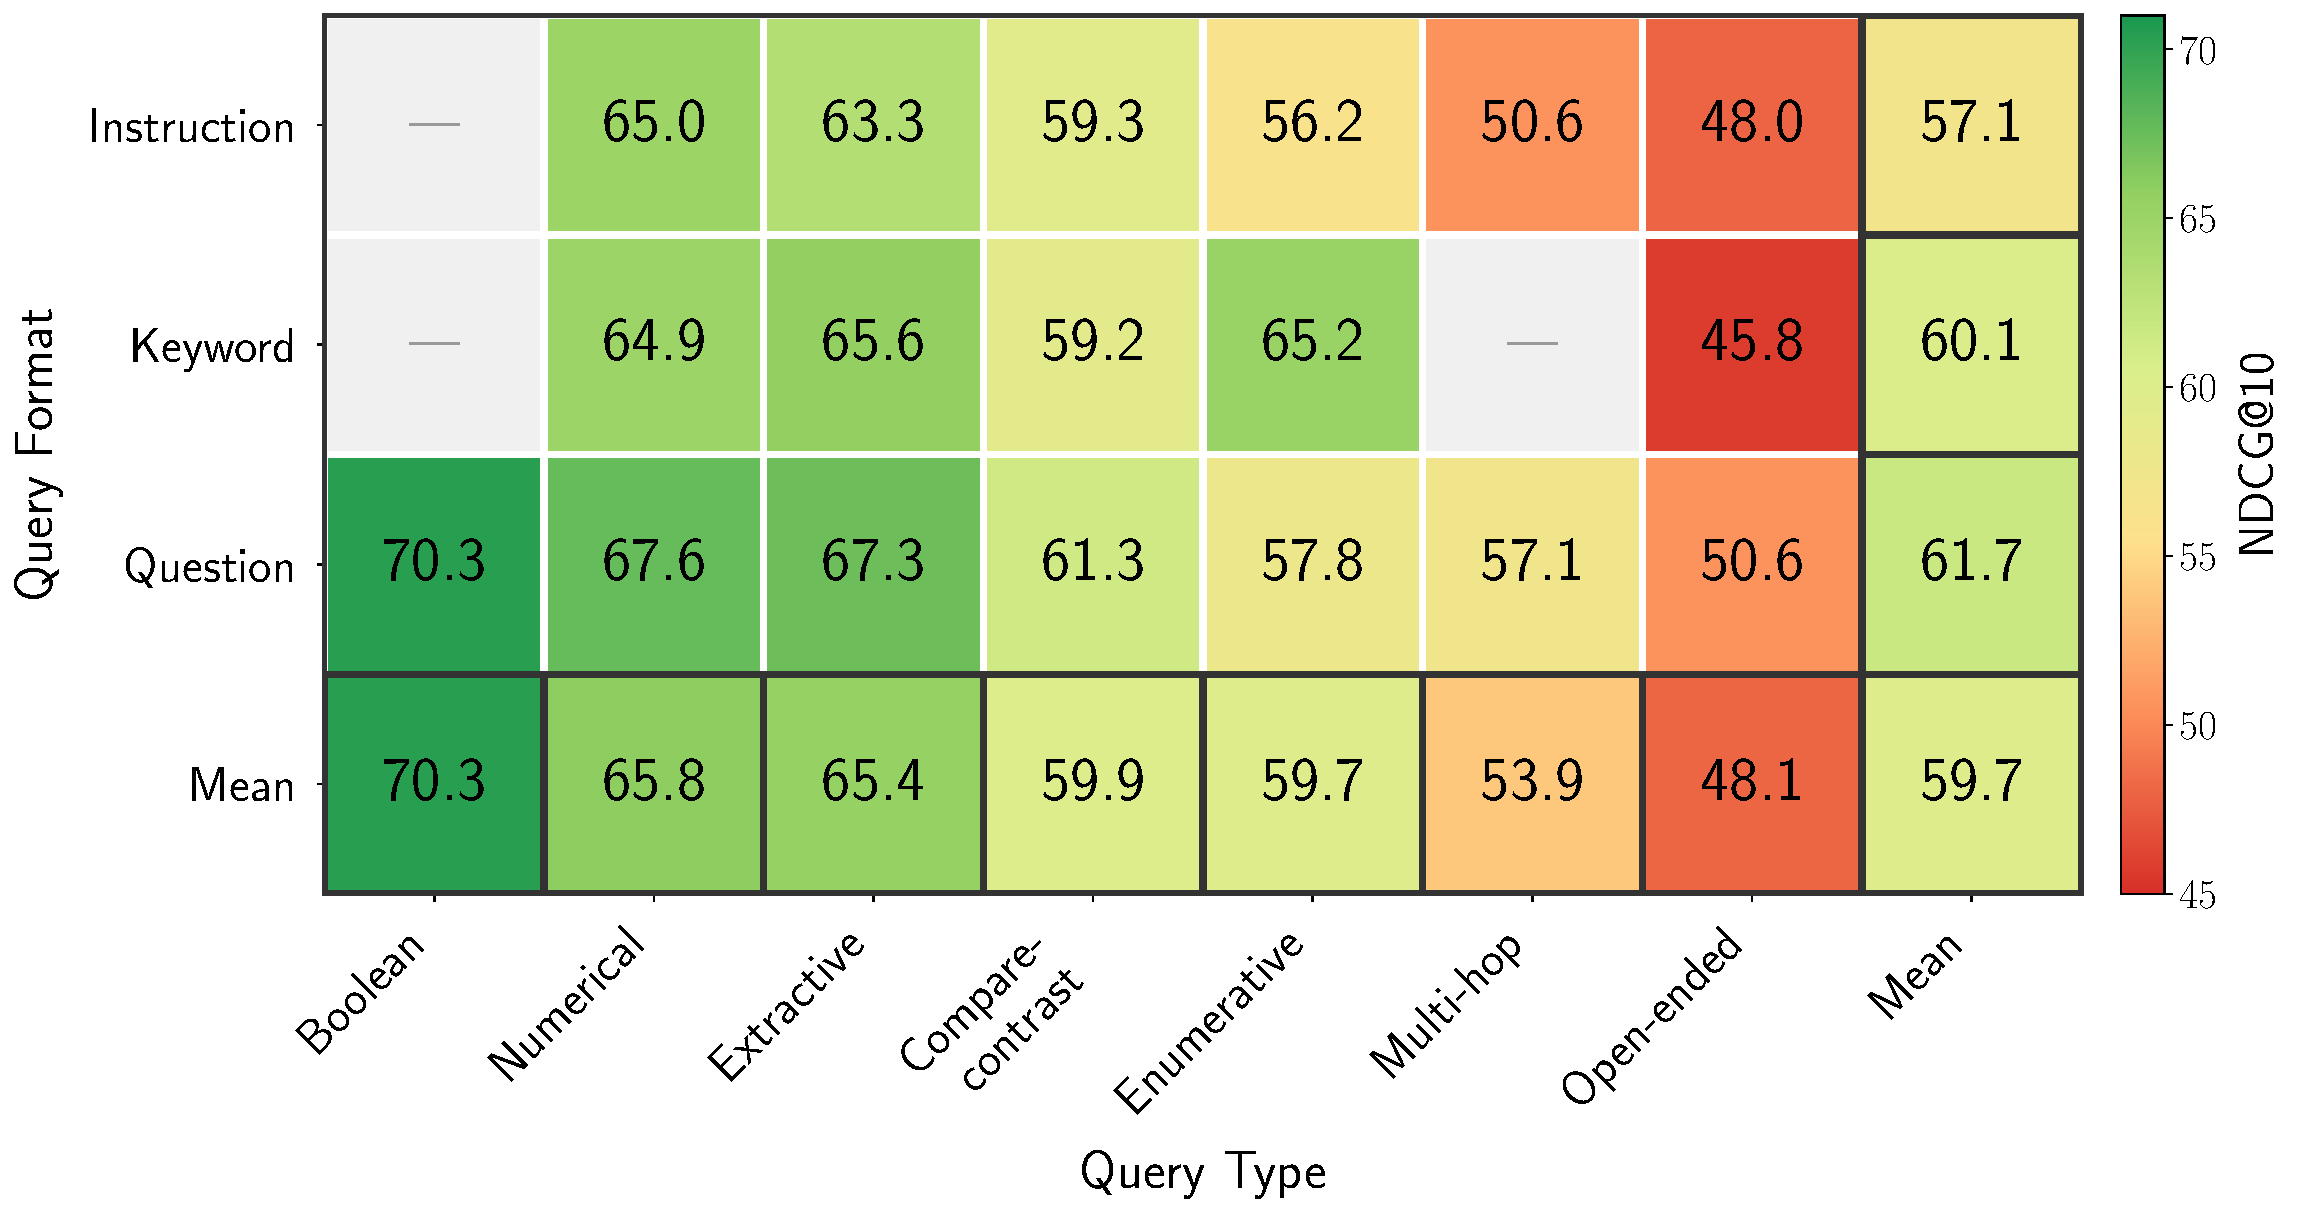
\includegraphics[width=0.99\columnwidth]{images/vidorev3_images/ndcg_by_type_format_transposed.pdf}
    \caption{\textbf{ColEmbed-3B-v2 NDCG@10 by query type and format.}}
    \label{fig:type-format-performance}
\end{figure}

% \begin{table}[h!]
% \centering
% % \resizebox{\columnwidth}{!}{%
% \begin{tabular}{lcc}
% \toprule
% Number of pages & NDCG@10 & Query count \\
% \midrule
% 1 & 76.4 & 4794 \\
% 2 & 64.7 & 3234 \\
% 3 & 60.5 & 1902 \\
% 4 & 58.7 & 1560 \\
% 5-9 & 48.5 & 4398 \\
% 10-19 & 41.2 & 2280 \\
% 20+ & 39.0 & 426 \\
% \bottomrule
% \end{tabular}
% % }
% \caption{\textbf{ColEmbed-3B-v2 NDCG@10 by number of annotated pages.}}
% \label{tab:perf number of pages}
% \end{table}

\paragraph{Visual Content and multi-page queries are hardest for retrievers}
\Cref{fig:content-type-performance} highlights that queries involving visual content like tables or images tend to be more difficult. The Mixed content type scores the lowest, which suggests that integrating information across different modalities within a single page remains a challenge. Additionally, we observe a consistent decline in performance as the number of annotated pages increases (\Cref{fig:perf number of pages}), suggesting that retriever effectiveness decreases
%when queries require aggregating information from multiple diverse sources.
when aggregating information from multiple sources is required.%\vic{think about whether this is normal for ndcg irrespective of query difficulty?} \manu{good point, not sure it's completely comparable even though ndcg is a measure of how perfect the ranking i}.

\begin{figure}[ht]
    \centering
    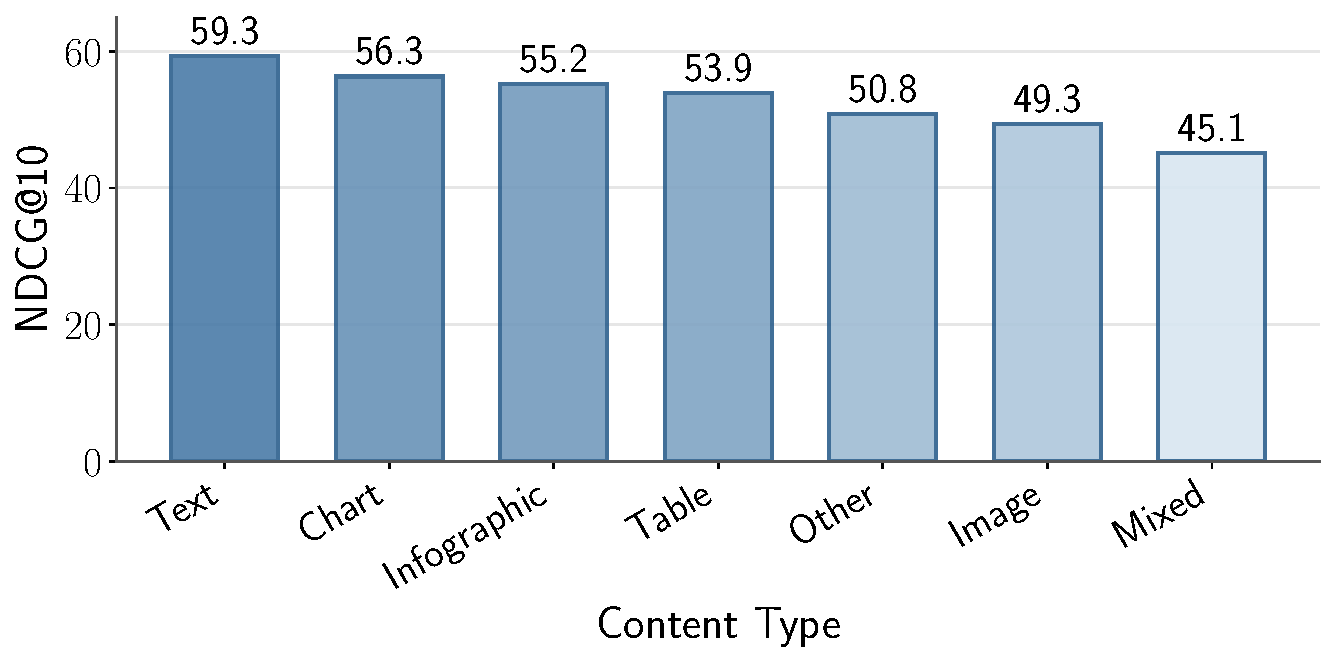
\includegraphics[width=\columnwidth]{images/vidorev3_images/ndcg_by_content_type.pdf}
    \caption{\textbf{ColEmbed-3B-v2 NDCG@10 by modality.}} 
    \label{fig:content-type-performance}
\end{figure}

\begin{figure}[h!]
    \centering
    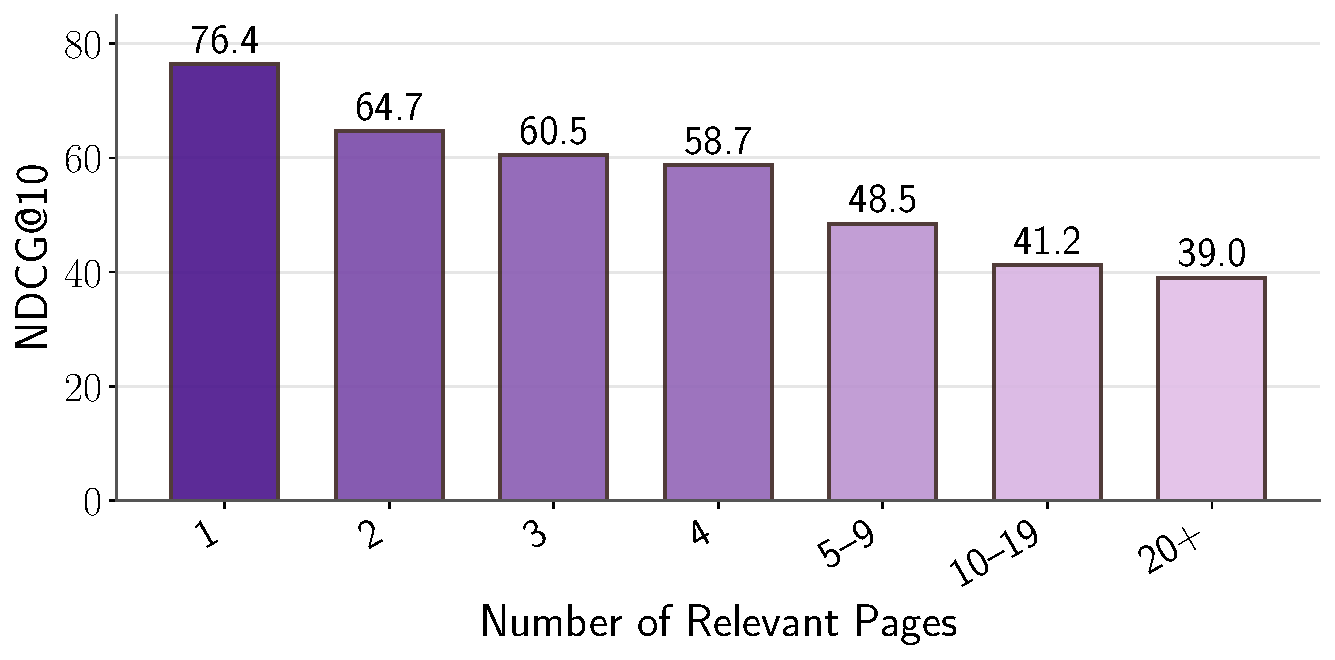
\includegraphics[width=\columnwidth]{images/vidorev3_images/ndcg_by_relevant_pages.pdf}
    \caption{\textbf{ColEmbed-3B-v2 NDCG@10 by number of annotated pages.}} 
    \label{fig:perf number of pages}
\end{figure}

\paragraph{Cross-language queries degrade performance}
Retrieval performance is 2--3 points higher in mono-lingual settings (\Cref{tab: english-only retrieval} and \Cref{tab: french-only retrieval}) than cross-lingual settings (\Cref{tab:retriever_comparison_updated}), showing that models need to better adapt to these settings. %\anto{Not super interesting}

%Retrieval performance is consistent across all 6 query languages (Table~\ref{tab:perf language}), with a 2.9 point NDCG@10 difference between the best (English, 60.8) and worst (German, 57.9) performers. However, we observe a small multilingual gap: NDCG@10 scores for English and French datasets are 2--3 points higher in a monolingual setting, where queries are in the same language as the documents (Tables~\ref{tab: english-only retrieval} and~\ref{tab: french-only retrieval}).

% \begin{figure}[ht]
%     \centering
%     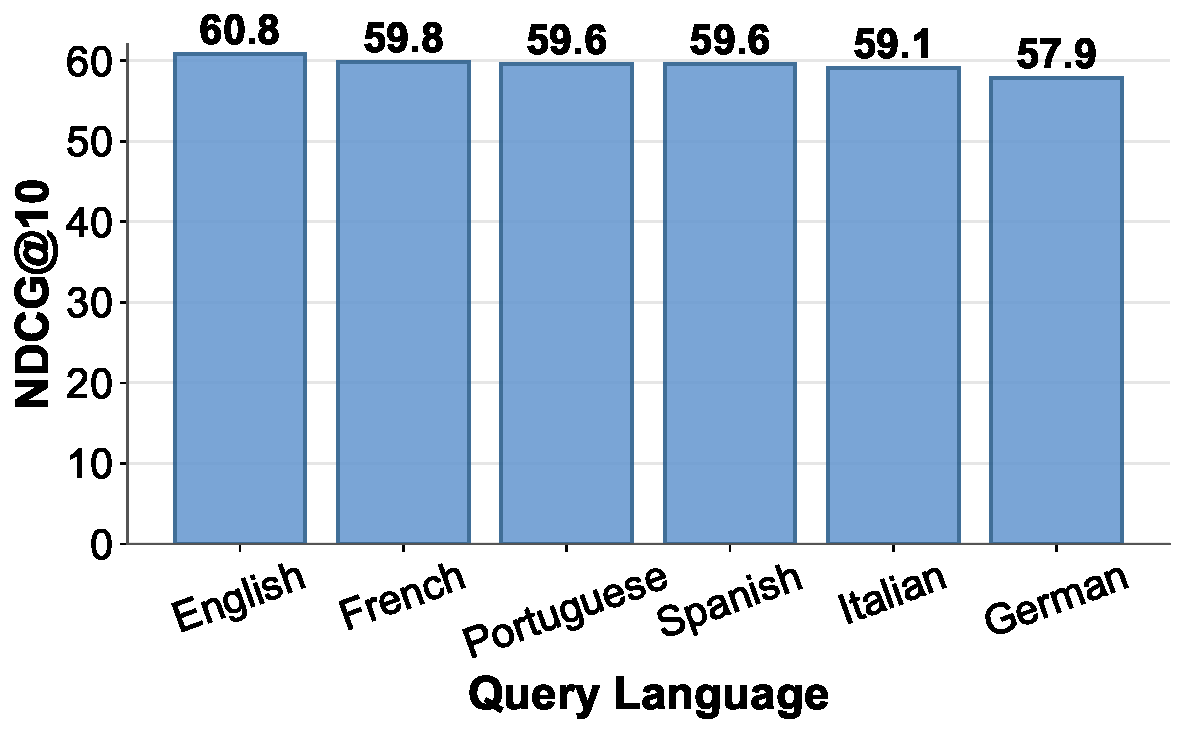
\includegraphics[width=\columnwidth]{images/vidorev3_images/ndcg_by_language.pdf}
%     \caption{ColEmbed-3B-v2 NDCG@10 by language.} 
%     \label{fig:size-performance}
% \end{figure}

\newcommand{\plus}[1]{\textcolor{teal}{\tiny \textbf{$\uparrow$#1}}}
\newcommand{\minus}[1]{\textcolor{red}{\tiny \textbf{$\downarrow$#1}}}
\newcommand{\val}[2]{\shortstack{#1 \\[-0.2em] \hspace{1.3em}#2}}
\newcommand{\dline}[2]{\shortstack{#1\\#2}}
\begin{table*}[h]
    \centering
    \small 
    \setlength{\tabcolsep}{3pt} 
    \resizebox{\textwidth}{!}{%
    \begin{tabular}{l ccccccc ccc >{\columncolor{avgcol}}c}
        \toprule
         & \multicolumn{7}{c}{\textbf{English Datasets}} & \multicolumn{3}{c}{\textbf{French Datasets}} & \multicolumn{1}{c}{} \\
        \cmidrule(lr){2-8} \cmidrule(lr){9-11}
        \textbf{Model}& \shortstack{C.S.} & \shortstack{Nucl.} & \shortstack{Fin.} & \shortstack{Phar.} & \shortstack{H.R.} & \shortstack{Ind.} & \shortstack{Tel.} & \shortstack{Phys.} & \shortstack{Ener.} & \shortstack{Fin.} & \textbf{Avg.} \\
        \midrule
        \textit{\textbf{Textual pipeline}} & \multicolumn{11}{c}{}\\
        \multirow[c]{2}{*}{\makecell[l]{Jina-v4\textsuperscript{textual} \\+ zerank-2}} &
        64.3 & 44.3 & 48.4 & 54.9 & 52.8 & 38.4 & 56.3 & 43.6 & 60.1 & 41.3 & 50.4 \\
         &
        \val{\textbf{82.1}}{\plus{17.8}} &
        \val{\textbf{53.5}}{\plus{9.2}} &
        \val{\textbf{69.2}}{\plus{20.8}} &
        \val{\textbf{66.2}}{\plus{11.3}} &
        \val{\textbf{66.5}}{\plus{13.7}} &
        \val{\textbf{53.2}}{\plus{14.8}} &
        \val{\textbf{71.5}}{\plus{15.2}} &
        \val{\textbf{48.2}}{\plus{4.6}} &
        \val{\textbf{71.5}}{\plus{11.4}} &
        \val{\textbf{53.7}}{\plus{12.4}} &
        \val{\textbf{63.6}}{\plus{13.2}} 
        \\
        \midrule
        \textit{\textbf{Visual pipeline}} & \multicolumn{11}{c}{} \\
        \multirow[c]{2}{*}{\makecell[l]{Jina-v4\textsuperscript{visual} \\+ jina-reranker-m0}} & 71.8 & 50.0 & 59.3 & 63.1 & 59.5 & 50.4 & 64.8 & 46.6 & 64.0 & 46.1 & 57.6 \\
        &
        \val{76.7}{\plus{4.9}} & 
        \val{50.8}{\plus{0.8}} & 
        \val{59.2}{\minus{0.1}} & 
        \val{65.4}{\plus{2.3}} & 
        \val{56.0}{\minus{3.5}} & 
        \val{50.9}{\plus{0.5}} & 
        \val{70.8}{\plus{6.0}} & 
        \val{46.9}{\plus{0.3}} & 
        \val{61.7}{\minus{2.3}} & 
        \val{39.8}{\minus{6.3}} & 
        \val{57.8}{\plus{0.2}} \\
        \bottomrule
    \end{tabular}
    }
    \caption{\textbf{Retrieval performance (NDCG@10) of retriever + reranker pipelines.}}
    \label{tab:reranking_scores_stacked}
\end{table*}

% \que{Condensed version but not a big fan} \paragraph{Textual rerankers help significantly; visual rerankers need improvement.} We test zerank-2 \sidecite{zeroentropy2025} and jina-reranker-m0 \sidecite{jinareranker2025} atop Jina-v4. Table~\ref{tab:reranking_scores_stacked} reveals a performance gap: though the visual base is stronger, the textual reranker yields substantial gains (+13.2 NDCG@10), outperforming the visual pipeline. Meanwhile, the visual reranker provides a marginal +0.2 average improvement and degrades performance across 4 datasets, necessitating better multilingual visual rerankers.

\paragraph{Textual rerankers outperform visual ones}

We evaluate the impact of adding a reranker to the textual and visual pipelines of the Jina-v4 retriever. We select zerank-2 \sidecite{zeroentropy2025} and jina-reranker-m0 \sidecite{jinareranker2025} as two of the leading textual and visual rerankers to date. Results in Table~\ref{tab:reranking_scores_stacked} reveal a significant disparity in reranking efficacy between modalities. While the visual retriever initially outperforms the textual base, the textual reranker yields substantial gains (+13.2 NDCG@10), enabling the textual pipeline to achieve the highest overall retrieval performance. In contrast, the visual reranker provides only a marginal average improvement of +0.2 and degrades performance in 4 datasets, underscoring the need for better multilingual visual rerankers.

%\gmor{When you evaluate with jina embedding v4 for text and image, do you use single-vector or late-interaction (as it supports both)? It is harder for cross-encoder to improve results from late interaction embedding model.}

\begin{table*}[h!]
\centering
\small
\resizebox{\textwidth}{!}{%
\begin{tabular}{l l l ccccc ccc >{\columncolor{avgcol}}c c c}
\toprule
& & & \multicolumn{5}{c}{\textbf{English Datasets}} & \multicolumn{3}{c}{\textbf{French Datasets}} & \cellcolor{white}& & \cellcolor{white} \\
\cmidrule(lr){4-8} \cmidrule(lr){9-11}
\makecell[l]{\textbf{Retrieval} \\ \textbf{pipeline}} & \makecell[l]{\textbf{Context} \\ \textbf{modality}} & \makecell[l]{\textbf{Generation} \\ \textbf{model}} & \makecell{C.S.} & \makecell{Fin.} & \makecell{Phar.} & \makecell{H.R.} & \makecell{Ind.} & \makecell{Phys.} & \makecell{Ener.} & \makecell{Fin.} & \makecell{\textbf{Avg.}\\\textbf{Hard}}& \makecell{Avg.\\Easy} & \makecell{Avg.\\Global} \\
\midrule
\multirow{3}{*}{Oracle} & Text & \multirow{3}{*}{Gemini 3 Pro} & 80.9 & 70.2 & 71.4 & \textbf{72.3} & 66.4 & 71.2 & 69.2 & 62.8 & 62.3& 79.3 & 70.6 \\
& Image & & \textbf{86.5} & \textbf{70.6} & \textbf{76.1} & 71.1 & \textbf{68.2} & 74.5 & \textbf{69.8} & \textbf{64.1} & \textbf{64.7}& \textbf{79.7} & \textbf{72.6} \\
& Hybrid & & 86.0 & 68.9 & 73.4 & 70.4 & 65.4 & 69.2 & 69.5 & 62.8 & 63.4& 77.5 & 70.7 \\
\midrule
\makecell[l]{Jina-v4\textsuperscript{text.} + zerank-2} & Text & Gemini 3 Pro & 80.9 & 66.0 & 59.9 & 63.2 & 60.4 & 69.2 & 64.9 & \underline{54.7} & 52.1& 75.5 & 64.9 \\
% \midrule
% Jina-v4\textsuperscript{text.} \& Jina-v4\textsuperscript{vis.} & Hybrid & Gemini 3 Pro & 82.8 & 62.1 & 59.6 & 61.6 & 57.2 & 64.9 & 61.4 & 51.2 & 62.6 & 71.7 & 52.2 \\
\midrule
\makecell[l]{Jina-v4\textsuperscript{text.} + zerank-2 \\ \& ColEmbed-3B-v2} & Hybrid & Gemini 3 Pro & 85.1 & 65.0 & 65.9 & 64.8 & 59.4 & 69.9 & 62.7 & 52.8 & \underline{54.7}& 76.6 & 65.7 \\
\midrule
\multirow{6}{*}{ColEmbed-3B-v2} & \multirow{2}{*}{Text} & Gemini 3 Pro & 82.3 & 62.5 & 61.0 & 62.9 & 56.2 & 64.9 & 62.3 & 49.4 & 51.7& 73.0 & 62.7 \\
 & & Kimi K2 & 81.4 & 56.6 & 59.1 & 55.7 & 55.8 & 73.8 & 60.4 & 43.1 & 44.6& 74.3 & 60.7 \\
\cmidrule{2-14}
& \multirow{4}{*}{Image} & Gemini 3 Pro & 83.3 & \underline{67.3} & 62.9 & 65.4 & 57.2 & 67.9 & 64.3 & 47.8 & 54.5& 74.1 & 64.5 \\
 & & Gemini 3 Flash & 80.9 & 64.1 & 63.5 & 63.8 & 55.1 & 68.2 & 63.3 & 47.8 & 50.3& 74.4 & 63.3 \\
& & GPT-5.2 & \underline{\textbf{86.5}} & 59.5 & \underline{68.1} & \underline{66.0} & \underline{61.5} & \underline{\textbf{76.5}} & \underline{66.2} & 49.1 & 54.1& \underline{78.1} & \underline{66.7} \\
& & Qwen3-VL-235B & 86.0 & 59.9 & 64.0 & 60.7 & 57.2 & 71.9 & 59.7 & 44.4 & 51.0& 74.1 & 63.0 \\
\bottomrule
\end{tabular}
}
\caption{\textbf{End-to-end evaluation of final answer generation.} We report the percentage of correct final answers as determined by an LLM judge across the 8 public datasets. "Oracle" rows represent the upper-bound performance using gold-standard contexts. Average Easy and Average Hard denote performance stratified by query difficulty. For each column, the best result is \textbf{bolded} and the best non-oracle result is \underline{underlined}.} % We systematically evaluate the effect of the retrieval pipeline, context modality, and generation model on the generation performance.
\label{tab:end_to_end_eval}
\end{table*}


\subsection{Final Answer Generation} \label{sec:answer results}

We evaluate end-to-end answer quality by providing LLMs and VLMs with queries and their corresponding retrieved pages, examining the effects of retrieval pipeline selection, context modality, and generation model choice (\Cref{tab:end_to_end_eval}). For this evaluation, we use the best-performing textual and visual retrieval pipelines. We additionally establish an upper bound using an \textit{oracle} pipeline that supplies the model with ground-truth annotated pages.

% For this evaluation, we use the best-performing textual and visual retrieval pipelines under 3B parameters
% -> no more reasons to say that right?

In the \textit{hybrid} configuration, we concatenate the top-5 results from the visual retriever (images) with the top-5 results from the textual retriever (text), without removing duplicates; the retrieval performance is detailed in \Cref{tab:hybrid_comparison}. We also consider a hybrid \textit{oracle} setup, which provides the model with all the ground-truth pages in both modalities.

%We evaluate the quality of final answers generated by LLMs when provided with a query and its relevant retrieved pages, assessing the impact of the retrieval pipeline, context modality, and generation model (\Cref{tab:end_to_end_eval}). We use the best-performing textual (Jina-v4) and visual (ColEmbed-3B-v2) pipelines under 3B parameters for this end-to-end evaluation. An \textit{oracle} pipeline, where the model receives the ground truth annotated pages, serves as an upper bound baseline.

The correctness of generated answers is assessed against the ground truth final answer by an LLM judge (details in Appendix \ref{appendix:final answer eval}). 
%Details on the evaluation setup are given in Appendix~\ref{appendix:final answer eval}.
Private datasets are omitted 
%from this evaluation
to maintain their integrity.

Some benchmark queries involve general knowledge manageable by LLMs without retrieval. To prevent memorization from confounding our assessment of the RAG pipeline, we stratify queries by difficulty based on parametric knowledge. A query is categorized as \textit{easy} if any model in a 6-LLM panel answers it correctly without context; otherwise, it is labeled \textit{hard}. Overall, 48.6\,\% of queries are easy (see~\Cref{tab: easy hard filtering} for details).

% A subset of queries in our benchmark can be answered by LLMs without retrieval, as they pertain to general knowledge that they already master. For these queries, high answer accuracy may reflect memorization rather than effective use of retrieved context, confounding our ability to assess the retrieval-augmented generation pipeline. To address this, we stratify queries by difficulty based on whether state-of-the-art LLMs can answer them from parametric knowledge alone. Specifically, we categorize a query as \textit{easy} if any model in a panel of 6 different LLMs answers it correctly without retrieved context; the remaining queries are labeled \textit{hard}. In total, 48.6\,\% of the queries fall into the easy category (see ~\Cref{tab: easy hard filtering} for a breakdown by dataset and panel model).

\paragraph{Visual context helps generation} With a fixed Gemini 3 Pro generator, image-based context outperforms text-based context on the hard subset by 2.4 and 2.8 percentage points for the oracle and ColEmbed-3B-v2 pipelines, respectively (\Cref{tab:end_to_end_eval}). This confirms that preserving the visual content of document pages provides better grounding for complex answer generation.

% \manu{check bold takeaway formatting}

%\paragraph{Generation quality reflects retrieval performance} Performance differences between retrieval pipelines persist in final answer quality. Notably, a strong textual pipeline (jina-embeddings-v4+zerank-2) can match a visual pipeline (colembed-3b-v2), achieving 64.9\% versus 64.5\% accuracy \que{TODO : rather talk about hard subset}. 
% \gmor{We might add a comment that for hard questions visual retrieval with ColEmbed-3B-v2 is better (54.5) than Jina text embedding+reranker pipeline (52.2)} 
%The 6 percentage point gap between oracle and the best retrieval pipelines highlights the effect of retrieval errors on final answer quality. % TODO: Rework this paragraph. The message is not well supported

\paragraph{Hybrid retrieval yields the best performance on challenging queries} The hybrid pipeline achieves 54.7\,\% accuracy on hard queries, surpassing both the strongest textual (52.1\,\%) and visual (54.5\,\%) baselines. This complementary effect suggests that text and image representations capture different aspects of document content, and their combination can provide more robust evidence for downstream generation. %\que{Not sure about last sentence, seems difficult to back} Conversely, the hybrid oracle (63.4\,\%) trails the image-only upper bound (64.7\,\%), indicating that the redundancy beneficial for retrieval robustness effectively dilutes the signal compared to pure visual grounding.

\paragraph{Hard queries expose the limits of parametric knowledge in current models} Even with oracle context, performance on hard queries lags behind easy queries by more than 10 percentage points. This gap suggests that the multi-step reasoning and long-context synthesis required for difficult queries remain challenging for current models. While the models we evaluate achieve comparable overall scores, their relative ranking may shift when parametric knowledge is less of an advantage, as shown by GPT 5.2 outperforming Gemini 3 Pro on easy queries but trailing on hard ones.

%\paragraph{Query difficulty is the main driver of performance variation} \anto{Don't like this sentence} Even with oracle context, performance on hard queries lags behind easy queries by more than 10 percentage points. This gap suggests that the multi-step reasoning and long-context synthesis required for difficult queries remain challenging for current models. While the models we evaluate achieve comparable overall scores, their relative ranking may shift when parametric knowledge is less of an advantage, as shown by GPT 5.2 outperforming Gemini 3 Pro on easy queries but trailing on hard ones.

\paragraph{ViDoRe V3 leaves significant room for future retriever improvements} The 10-point gap between the best non-oracle result (54.7\,\%) and the image oracle (64.7\,\%) on hard queries underscores substantial opportunities for improving the retrieval pipeline. Moreover, even with oracle contexts, Gemini 3 Pro performance remains modest, indicating that generation models still struggle to fully exploit the provided information.

%\paragraph{Generation quality reflects retrieval performance} \aedy{either change name or takeaway} Performance differences between retrieval pipelines persist in final answer quality. While the best textual (jina-embeddings-v4+zerank-2) and visual (colembed-3b-v2) pipelines show comparable overall averages, a distinct advantage for visual retrieval emerges on the hard subset (+2.4\,\%). The significant 10-point gap between the best non-oracle result (54.7\,\%) and the image oracle (64.7\,\%) on hard queries highlights the substantial room for improvement in retrieval pipelines.


% \begin{table*}[h]
% \centering
% \label{tab:ragchecker_metrics}
% \resizebox{\textwidth}{!}{%
% \begin{tabular}{l|ccc|cc|cccccc}
%  & \multicolumn{3}{c}{\textit{Overall}} & \multicolumn{2}{c}{\textit{Retriever}} & \multicolumn{6}{c}{\textit{Generator}} \\
% \midrule
% Domaine & Precision $\uparrow$ & Recall $\uparrow$ & F1 $\uparrow$ & \dline{Claim}{Recall} $\uparrow$ & \dline{Context}{Precision} $\uparrow$ & \dline{Context}{Utilisation} $\uparrow$ & \dline{Noise}{Sensitivity (R)} $\downarrow$& \dline{Noise}{Sensitivity (I)} $\downarrow$ & Hallu. $\downarrow$ & \dline{Self}{Knowledge} $\downarrow$ & Faith. $\uparrow$\\
% \midrule
% Computer Science & 70.9 & 68.2 & 60.2 & 89.9 & 85.0 & 70.7 & 18.1 & 1.4 & 9.6 & 4.0 & 86.3 \\
% Energy (FR) & 62.6 & 65.6 & 55.1 & 81.2 & 75.7 & 66.6 & 20.2 & 4.7 & 12.5 & 5.7 & 81.9 \\
% Finance (EN) & 63.8 & 52.7 & 47.9 & 85.8 & 71.3 & 52.0 & 17.2 & 5.1 & 13.9 & 5.3 & 80.9 \\
% Finance (FR) & 51.3 & 55.5 & 43.0 & 76.9 & 68.3 & 54.2 & 25.3 & 7.1 & 16.4 & 5.8 & 77.8 \\
% HR (EN) & 65.5 & 56.7 & 50.7 & 80.9 & 66.2 & 55.3 & 18.1 & 3.8 & 12.6 & 6.5 & 80.9 \\
% Industrial (EN) & 63.7 & 58.2 & 49.6 & 85.4 & 76.4 & 59.3 & 20.7 & 4.7 & 11.0 & 5.9 & 83.2 \\
% Pharmaceuticals (EN) & 62.5 & 65.8 & 55.1 & 82.2 & 73.6 & 64.7 & 19.8 & 3.4 & 14.2 & 9.7 & 76.0 \\
% Physics (FR) & 63.2 & 65.8 & 55.0 & 74.0 & 74.0 & 68.1 & 14.8 & 2.7 & 19.2 & 13.4 & 67.4 \\
% \midrule
% Mean & 62.9 & 61.1 & 52.1 & 82.0 & 73.8 & 61.4 & 19.3 & 4.1 & 13.7 & 7.0 & 79.3 \\
% \midrule
% Easy queries & 63.6 & 65.6 & 53.8 & 86.0 & 76.9 & 66.2 & 21.2 & 2.8 & 12.4 & 6.8 & 80.8 \\
% Hard queries & 62.0 & 55.8 & 49.6 & 79.1 & 71.1 & 55.7 & 18.1 & 5.2 & 14.7 & 6.8 & 78.4 \\
% \bottomrule
% \end{tabular}%
% }
% \caption{RAGChecker Metrics across Datasets, for Oracle retriever + gpt-5 \aedy{wdyt}\\ \aedy{METRICS: https://github.com/amazon-science/RAGChecker}}
% \end{table*}

\subsection{Visual Grounding} \label{sec:visual grounding results}

Beyond generating correct answers, it is highly desirable for RAG pipelines to identify where in the source documents the answer originates, enabling users to verify the grounding of the query answer. We therefore evaluate the ability of LLMs to generate accurate bounding boxes within their final answer. Among the few LLM families with visual grounding capabilities, we select Qwen3-VL-30B-A3B-Instruct and Gemini 3 Pro for evaluation. For each query, we provide the model with the candidate pages shown to the human annotators and prompt it to answer the query while inserting inline bounding boxes in XML format \texttt{<bboxes image="N"> ... </bboxes>} to delimit relevant content (full instructions in Appendix~\ref{appendix: bbox}).

We use the bounding boxes produced by the human annotators as our ground truth. Since each query may have 1--3 human annotators, we evaluate VLM predictions independently against each annotator using the same zone-based methodology as the inter-annotator consistency analysis (Section~\ref{sec: grounded qa}), and report the highest F1 score. This best-match strategy reflects the inherent subjectivity of evidence selection: annotators may legitimately highlight different regions to support the same answer, and a model should not be penalized for matching any valid interpretation.

% \begin{table}[h!]
% \centering
% \footnotesize
% \setlength{\tabcolsep}{6pt}
% \begin{tabular}{@{}lc@{}}
% \toprule
% Predictor & F1 \\
% \midrule
% Qwen3-VL-30B-A3B & 0.089 \\
% Gemini 3 Pro & 0.065 \\
% \addlinespace[0.2em]
% \textit{Human Agreement} & \textit{0.602} \\
% \bottomrule
% \end{tabular}
% \caption{Average Localization F1 scores.}
% \label{tab:bbox_f1}
% \end{table}

\paragraph{Visual grounding lags human performance} 
Inter-annotator agreement on evidence localization reaches an F1 of 0.602, whereas the best-performing models achieve markedly lower scores: 0.089 for Qwen3-VL-30B-A3B-Instruct and 0.065 for Gemini 3 Pro. A page-level analysis (\Cref{tab:bbox_consistency_comparison}) reveals that on pages where humans provided bounding boxes, both models annotated the same page only 16--17\,\% of the time, while 26--27\,\% of human-annotated pages received no model annotation at all—highlighting recall as the primary bottleneck. Detailed per-domain results and qualitative analysis appear in Appendix \ref{appendix: bbox} and \ref{appendix: bbox examples}.

%Table~\ref{tab:bbox_consistency_comparison} provides a page-level analysis of annotation presence: on pages where humans provided bounding boxes, both models annotated the same page only 16--17\,\% of the time, while 26--27\,\% of human-annotated pages received no model annotation at all, highlighting recall as the primary limitation. Localization F1 scores (Figure~\ref{fig:bbox evaluation}) reveal that the models score substantially below inter-annotator agreement (Table~\ref{tab:inter-annotator bbox agreement}). Qualitative analysis reveals distinct failure modes (examples in Appendix~\ref{appendix: bbox examples}). Gemini frequently produces off-by-one page indexing errors: the predicted coordinates would correctly localize the target content if applied to an adjacent page. The two models also differ in box granularity: Gemini tends to draw tight boxes around individual elements (e.g., a single table cell or text line), whereas Qwen3-VL generates larger boxes encompassing entire sections or paragraphs, more closely matching human annotation patterns \gmor{If we need to save some space for submission, these details about how Gemini and Qwen3-VL generates boxes could go to the Appendix}. This difference partially explains Qwen3-VL's higher F1 scores, as broader boxes are more likely to overlap with the ground-truth zones used in our evaluation.

% \paragraph{Agreement-Based Stratification}
% To understand how VLM performance varies with annotation ambiguity, we stratify results by inter-annotator agreement level. For multi-annotator samples, we compute pairwise zone IoU between all annotator pairs and classify agreement as \textit{high} (mean pairwise IoU $\geq 0.7$), \textit{medium} ($0.3 \leq$ IoU $< 0.7$), \textit{low} (IoU $< 0.3$), or \textit{single} (one annotator only).


% \begin{table*}[h!]
% \centering
% \small 
% \setlength{\tabcolsep}{3pt} 
% % \resizebox{\textwidth}{!}{%
% \begin{tabular}{l ccccccc ccc c} % Removed columncolor from here
% \toprule
%  & \multicolumn{7}{c}{\textbf{English Datasets}} & \multicolumn{3}{c}{\textbf{French Datasets}} & \\ % This cell is now white
% \cmidrule(lr){2-8} \cmidrule(lr){9-11}
% \makecell[l]{\textbf{Model}} & \makecell{C.S.} & \makecell{Nucl.} & \makecell{Fin.} & \makecell{Phar.} & \makecell{H.R.} & \makecell{Ind.} & \makecell{Tel.} & \makecell{Phys.} & \makecell{Ener.} & \makecell{Fin.} & \makecell{\textbf{Average}} \\
% \midrule
% Qwen3-VL-30B-A3B & 0.058 & 0.094 & 0.050 & 0.157 & 0.054 & 0.066 & 0.078 & 0.198 & 0.086 & 0.044 & \cellcolor{avgcol}\textbf{0.084} \\
% Gemini 3 Pro & 0.055 & 0.070 & 0.036 & 0.103 & 0.036 & 0.035 & 0.073 & 0.144 & 0.067 & 0.028 & \cellcolor{avgcol}\textbf{0.061} \\
% \bottomrule
% \end{tabular}
% %}
% \caption{\textbf{Model bounding box localization performance}. Each F1 score measures the zone-based overlap between model-generated bounding boxes and human annotations, using the annotator yielding the highest F1.\vic{Transform into graph to make this more legible?}}
% \label{tab:bbox evaluation}
% \end{table*}


\begin{table}[h!]
\centering
\resizebox{\columnwidth}{!}{%
\begin{tabular}{llcc}
\toprule
\textbf{Category} & \textbf{Outcome} & \textbf{Qwen3-VL-30B-A3B} & \textbf{Gemini 3 Pro} \\
\midrule
\multirow{2}{*}{\textbf{Agreement}} 
  & Both annotated & 17\,\% & 16\,\% \\
  & Neither annotated  & 46\,\% & 49\,\% \\
\addlinespace
\multirow{2}{*}{\textbf{Discrepancy}} 
  & Model only   & 10\,\% & 7\,\% \\
  & Human only & 26\,\% & 27\,\% \\
\bottomrule
\end{tabular}
}
\caption{\textbf{Page-level bounding box agreement between models and human annotators.} Each page is classified by whether the model and human both annotated it, both left it unannotated, or only one provided annotations.}
\label{tab:bbox_consistency_comparison}
\end{table}



% \begin{table}[h!]
% \small
% \centering
% \resizebox{\columnwidth}{!}{%
% \begin{tabular}{lc}
% \toprule
% \textbf{Predictor} & \textbf{F1} \\
% \midrule
% Qwen3-VL-30B-A3B & 0.089 \\
% Gemini 3 Pro & 0.065 \\
% \hline
% Human & 0.602 \\
% \bottomrule
% \end{tabular}
% }
% \caption{\textbf{Average Localization F1 score over each corpus.}}
% \label{tab:bbox_f1}
% \end{table}


% \paragraph{Visual Document Understanding (VDU)} The field of VDU has traditionally relied on datasets such as DocVQA \sidecite{mathew_docvqa_2020} and CharXiv \sidecite{wang2024charxiv}. Such works are also often specialized in one particular document type \sidecite{mathew2021infographicvqa, zhu_towards_2022, tanaka2023slidevqa} While these benchmarks have been instrumental in advancing multimodal understanding, they are primarily designed for single-page or single-image tasks. They do not require the system to sift through large corpora, thereby bypassing the retrieval challenges inherent in RAG. Furthermore, recent efforts to introduce bounding box supervision, such as BBox-DocVQA \sidecite{yu2025bboxdocvqalargescale}, remain restricted to these single-page contexts and do not address multi-page retrieval scenarios.

% \paragraph{Retrieval-Centric Benchmarks} The rapid evolution of visual retrieval models \sidecite{yu2024visragvisionbasedretrievalaugmentedgeneration, ma2024unifyingmultimodalretrievaldocument}, particularly ColBERT style late-interaction architectures like ColPali \sidecite{faysse2025colpaliefficientdocumentretrieval, xu2025llamanemoretrievercolembedtopperforming}, has necessitated new evaluation frameworks. Benchmarks such as Jina-VDR \sidecite{günther2025jinaembeddingsv4universalembeddingsmultimodal} and ViDoRe V1/V2 \sidecite{faysse2025colpaliefficientdocumentretrieval, macé2025vidorebenchmarkv2raising} have been developed to measure retrieval precision. However, these benchmarks largely isolate the retrieval step. They overlook the subsequent generation phase, failing to evaluate whether the retrieved context is sufficient for a model to synthesize a coherent, grounded answer.

% \paragraph{End-to-End Multimodal RAG}
% While textual RAG benchmarks have recently evolved to capture realistic, non-trivial user needs \sidecite{thakur2025freshstackbuildingrealisticbenchmarks, tang2024multihopragbenchmarkingretrievalaugmentedgeneration, su2024bright}, this level of query complexity remains largely underexplored for multimodal RAG. In contrast, multimodal RAG evaluation still lacks this depth \sidecite{faysse2025colpaliefficientdocumentretrieval, wang2025vidorag, wasserman2025real}.Recent works like DUDE \sidecite{van2023document} and M3DocRAG \sidecite{cho2024m3docrag} extend evaluation to multi-page settings but remain heavily skewed toward extractive tasks. These datasets typically demand short, factoid answers that do not stress the multi-step reasoning or synthesis capabilities required by open-ended enterprise queries.The closest contemporary work, UniDocBench \sidecite{peng2025unidocbenchunifiedbenchmarkdocumentcentric}, offers a significant step toward end-to-end evaluation with tasks including summarization and reasoning. However, it relies heavily on synthetic generation with sparse human verification, is limited to a single language, and lacks the fine-grained visual grounding annotations necessary to diagnose hallucinations in complex layouts. Our work bridges these gaps by providing a multilingual, expert-verified benchmark that enforces visual grounding and targets complex, open-ended reasoning.

% \manu{Not sure this RW brings a lot compared to what is in the intro. Maybe call the intro "intro and Related Work" and add a few citations there. It seems quite redundant here.}

\section{Conclusion}

This work introduces ViDoRe V3, a multilingual, human-annotated RAG benchmark that evaluates retrieval, final answer generation, and visual grounding on large industry-relevant document corpora. We design a human-in-the-loop annotation methodology, deployed in a 12,000-hour annotation campaign, that produces diverse realistic queries paired with relevant pages, bounding boxes, and reference answers. Evaluating state-of-the-art RAG pipelines, we find that visual retrievers outperform textual ones, late interaction and textual reranking yield substantial gains, and visual context improves answer generation quality. Looking ahead, ViDoRe V3 highlights several concrete research directions for practical multimodal RAG. Retriever models still struggle on cross-lingual and open-ended queries requiring visual interpretation, while VLMs need improvement in answer generation from multi-page contexts as well as accurate visual grounding. By providing a rigorous framework for evaluating these limitations, ViDoRe V3 serves as a catalyst for the development of more robust, intelligent document understanding models.
